\documentclass[10pt]{article}

%Packages with options
\usepackage[english]{babel}
\usepackage[mathscr]{euscript}
\usepackage[margin = 1in]{geometry}
\usepackage[utf8]{inputenc}
\usepackage[small]{titlesec}

% Primary Packages
\usepackage{adjustbox}
\usepackage{amsmath}
\usepackage{amssymb}
\usepackage{amsthm}
\usepackage{bm}
\usepackage{commath}
\usepackage{chngcntr}
\usepackage{dsfont}
\usepackage{econometrics}
\usepackage{fancyhdr}
\usepackage{gensymb}
\usepackage{graphicx}
\usepackage{hyperref}
\usepackage{longtable}
\usepackage{marginnote}
\usepackage{mathtools}
\usepackage{natbib}
\usepackage{mdframed}
\usepackage{parskip}
\usepackage{setspace}
\usepackage{subfigure}
\usepackage{tabularx}
\usepackage{textcomp}

% Secondary Pacakges [need to be loaded later]
\usepackage{breqn}

% Setting up page style 
\pagestyle{fancy}
\setlength{\headheight}{23pt}
\renewcommand{\headrulewidth}{0pt}
\renewcommand{\sectionmark}[1]{%
\markboth{\thesection\quad #1}{}}
\fancyhead{}
\fancyhead[R]{\leftmark}
\fancyfoot{}
\fancyfoot[C]{\thepage}
\linespread{1}

%Change expectation and probability to doublescript
\renewcommand{\E}{\mathbb{E}}
\renewcommand{\P}{\mathbb{P}}


% Make capital vectors commands from econometrics packages
\newcommand{\vA}{\mathbf{A}}
\newcommand{\vB}{\mathbf{B}}
\newcommand{\vC}{\mathbf{C}}
\newcommand{\vD}{\mathbf{D}}
\newcommand{\vE}{\mathbf{E}}
\newcommand{\vF}{\mathbf{F}}
\newcommand{\vG}{\mathbf{G}}
\newcommand{\vH}{\mathbf{H}}
\newcommand{\vI}{\mathbf{I}}
\newcommand{\vJ}{\mathbf{J}}
\newcommand{\vK}{\mathbf{K}}
\newcommand{\vL}{\mathbf{L}}
\newcommand{\vM}{\mathbf{M}}
\newcommand{\vN}{\mathbf{N}}
\newcommand{\vO}{\mathbf{O}}
\newcommand{\vP}{\mathbf{P}}
\newcommand{\vQ}{\mathbf{Q}}
\newcommand{\vR}{\mathbf{R}}
\newcommand{\vS}{\mathbf{S}}
\newcommand{\vT}{\mathbf{T}}
\newcommand{\vU}{\mathbf{U}}
\newcommand{\vV}{\mathbf{V}}
\newcommand{\vW}{\mathbf{W}}
\newcommand{\vX}{\mathbf{X}}
\newcommand{\vY}{\mathbf{Y}}
\newcommand{\vZ}{\mathbf{Z}}

%Declare some shortcuts
\newcommand{\thetaH}{\hat{\theta}}
\newcommand{\thetaT}{\tilde{\theta}}
\newcommand{\nuH}{\hat{\nu}}
\newcommand{\nuT}{\tilde{\nu}}
\newcommand{\muH}{\hat{\mu}}
\newcommand{\sigmaH}{\hat{\sigma}}
\newcommand{\DeltaT}{\tilde{\Delta}}
\newcommand{\ris}{\rho_{i}^*}
\newcommand{\ind}{\mathds{1}}
\newcommand{\wcov}{\rightsquigarrow}
\newcommand{\PK}{(K)}
\newcommand{\andbox}{\hbox{ }\text{ and }\hbox{ }}


%Declate New Math Operators
\DeclareMathOperator{\argmax}{arg\,max}
\DeclareMathOperator{\argmin}{arg\,min}
\DeclareMathOperator{\cube}{Cub}
\DeclareMathOperator{\Do}{do}
\DeclareMathOperator{\err}{err}
\DeclareMathOperator{\id}{id}
\DeclareMathOperator{\Poisson}{Poisson}
\DeclareMathOperator{\polylog}{polylog}
\DeclareMathOperator{\supp}{supp}
\DeclareMathOperator{\sign}{sign}
\DeclareMathOperator{\Var}{Var}

\newcommand\numberthis{\addtocounter{equation}{1}\tag{\theequation}}

\newtheoremstyle{exampstyle}
  {1em plus .2em minus .1em}%   Space above
  {1em plus .2em minus .1em}%   Space below
  {} % Body font
  {} % Indent amount
  {\bfseries} % Theorem head font
  {.} % Punctuation after theorem head
  {.5em} % Space after theorem head
  {} % Theorem head spec (can be left empty, meaning `normal')


 {
    \theoremstyle{exampstyle}
    \newtheorem{assumption}{Assumption}
    \newtheorem*{assumption*}{Assumption}
    \newtheorem{specification}{Specification}
    \newtheorem*{specification*}{Specification}
    \newtheorem{definition}{Definition}
    \newtheorem*{definition*}{Definition}
    \newtheorem{example}{Example}
    \newtheorem*{example*}{Example}
    \newtheorem{remark}{Remark}
    \newtheorem*{remark*}{Remark}
 }

\newtheorem{theorem}{Theorem}
\newtheorem*{theorem*}{Theorem}
\newtheorem{lemma}{Lemma}
\newtheorem*{lemma*}{Lemma}
\newtheorem{prop}{Proposition}
\newtheorem*{prop*}{Proposition}
\newtheorem{corollary}{Corollary}
\newtheorem*{corollary*}{Corollary}

\newcommand{\blocktheorem}[1]{%
  \csletcs{old#1}{#1}% Store \begin
  \csletcs{endold#1}{end#1}% Store \end
  \RenewDocumentEnvironment{#1}{o}
    {\par\addvspace{1.5ex}
     \noindent\begin{minipage}{\textwidth}
     \IfNoValueTF{##1}
       {\csuse{old#1}}
       {\csuse{old#1}[##1]}}
    {\csuse{endold#1}
     \end{minipage}
     \par\addvspace{1.5ex}}
}
\blocktheorem{theorem}
\blocktheorem{assumption}
\blocktheorem{definition}
\blocktheorem{prop}
\blocktheorem{specification}
\raggedbottom

%Reset equation counters for each section
\counterwithin*{assumption}{section}
\counterwithin*{corollary}{section}
\counterwithin*{definition}{section}
\counterwithin*{equation}{section}
\counterwithin*{figure}{section}
\counterwithin*{footnote}{subsection}
\counterwithin*{lemma}{section}
\counterwithin*{prop}{section}
\counterwithin*{remark}{section}
\counterwithin*{specification}{section}
\counterwithin*{table}{section}
\counterwithin*{theorem}{section}

\title{Readings on ML and High-Dimensional Methods}
\author{Manu Navjeevan}
\date{\today}

\begin{document}
\maketitle
\tableofcontents
\newpage

\normalsize
%!TEX root = /Users/manunavjeevan/Desktop/Research/ML + Lasso/Annotated Literature Review/litNotesML.tex

\section{Generalized Random Forests; \textit{\small Susan Athey, Julie Tibshirani, Setfan Wager (AOS, 2018)}}
This paper can be found on ArXiv \href{https://arxiv.org/pdf/1610.01271.pdf}{here}.
\subsection{Introduction}
\begin{itemize}
	\item Random Forests first introduced by Breiman (2001)
	\item Used for conditional mean estimation. Given a data generating distribution for $(X_i, Y_i) \in \mathscr{X}\times\mathbb{R}$, want to estimate 
	\begin{equation}
		\mu(x) = \mathbb{E}[Y| X_i = x]
	\end{equation}
	\item Paper extends this to a flexible method for estimating any quantity $\theta(x)$ defined via local moment conditions. Specifically, given data $(X_i, O_i) \in \mathscr{X}\times\mathscr{O}$, we want forest based estimates of $\theta(x)$ defined by a local moment condition of the form 
	\begin{equation}\label{MC1}
		\mathbb{E}[\psi_{\theta(x), \nu(x)}(O_i)|X_i = x] = 0, \hbox{ }\text{ for all }x\in \mathscr{X}
	\end{equation}
	where $\psi(\cdot)$ is a score function and $\nu(\cdot)$ is an optional nuisance parameter.
	\begin{itemize}
		\item For example, if we model the distribution of $O_i$ conditional on $X_i$ to have a density $f_{\theta(x), \nu(x)}(\cdot)$ then the moment condition one with $\psi = \nabla \log f_{\theta(x), \nu(x)}(\cdot)$ ideintifies the local maximum likelihood 
		\item Substantive application involved heterogeneous treatment effect estimation with IV
	\end{itemize}
	\item Aim is to build a famly of non-parametric estimators that inherit desirable empirical properties of regression forests: stability, ease of use, flexible adaptation to different functional forms
	\item Regression forests typically understood as ensemble methods
	\begin{equation*}
		\hat{\mu}(x) = B^{-1} \sum_{b= 1}^B \hat{\mu}_b(x)
	\end{equation*}
	because individual trees have low bias but high variance, this averaging stabilizes predictions. 

	This method may not work as well when we are given moment conditions as in \ref{MC1}. Noisy solutions to moment equations are generally biased and averaging would do nothing to alleviate the bias.

	\item Cast forests as a type of adaptive locally weighted estimatior that first uses a forest to calculate a weighted set of neighbors for each test point $x$ and then solves a plug-in version of \ref{MC1} using these neighbors.
	\begin{itemize}
		\item Previously advocated by Hotheorn et. al (2004) in the context of survival analysis and by Meinshausen (2006) for quantile regression
		\item For conditonal mean estimation the averaging and weighting views of forests are equivalent, for moment conditions the weighting based perspective proves more effective
	\end{itemize}
	\item Bulk of this paper is devoted to theoretical analysis of generalized random forests
\end{itemize}
\subsubsection{Related Work}
\begin{itemize}
	\item Idea of local maximum likelihood has a long history. Core idea: when estimating parameters at a particular value of covariates, a kernel weighting function is used to place more weight on nearby observations in the covariate space. Paper replaces the kernel weighting function with forest based weights. 
	\begin{itemize}
		\item Weights dervied from the fraction of trees in which an observation appears in the same leag as the target value of the covariate vector.
		\item If the covariate space has more than a few dimensions kernel methods can suffer from curse of dimensionality.
	\end{itemize}
\end{itemize}
\subsection{Generalized Random Forests}
\begin{itemize}
	\item In the standard classification or regresion forests proposed by Breiman (2001), prediction for a particular point $x$ is determined by averaging predictions across an ensemble of different trees.
\end{itemize}
Suppose that we have $n$ independent and identically distributed samples, indeced $i = 1, \dots, n$. For each sample, access to an observable quantity $O_i$ that encodes information relevant to estimation $\theta(\cdot)$, along with a set of auxilary covariates $X_i$.
\begin{itemize}
	\item In the case of NPR; $O_i = \{Y_i\}, Y_i \in \mathbb{R}$, though in general it may contain richer information. 
	\begin{itemize}
		\item In the case of treatment effect estimation weith exogeneous treatment assignment, $O_i = \{Y_i, W_i\}$ where $W_i$ represents the treatment assignment.
	\end{itemize}
\end{itemize}
Given this type of data, the goal is to estimation solutions to local estimation equations of the form $\mathbb{E}[\psi_{\theta(x), \nu{x}}(O_i)|X_i = x] = 0$ (Eq. \ref{MC1}), for all $x \in \mathscr{X}$. We care about $\theta(x)$ and $\nu(x)$ is a nuisance parameter. 

One approach: Define some similarity weights $\alpha_i(x)$ that measure the relevance of the $i$-th training example to fitting $\theta(\cdot)$ at $x$ and then fit the target of interest via an empirical version of the estimation equation 
\begin{equation}\label{eq:mc_sample}
	\left(\hat{\theta}(x), \hat{\nu}(x)\right) \in \arg\min_{\theta,\nu}\left\{\left\Vert \sum_{i=1}^n \alpha_i(x)\psi_{\theta,\nu}(O_i)\right\Vert_2\right\}
\end{equation}
If the expresion has a unique root we can say that the estimators ``solve'' eq. \ref{eq:mc_sample}. Weights used in the above equations are traditionally obtained via a deterministic kernel function, perhaps with an adaptively chosen bandwith parameter. This method of choosing weights suffers from curse of dimensionality. This paper uses forest-based algorithms to adaptively learn better, problem specifc, weights, $\alpha_i(x))$ that van be used in conjunction with eq. \ref{eq:mc_sample}.
\begin{enumerate}
	\item Grow a set of $B$ trees indicated by $b=1, \dots, B$ and, for each such tree, define $L_b(x)$ as the set of training examples falling in the same ``leaf'' as $x$.
	\item Define the weights as the frequency with with the $i$-th training example falls into the same leaf as $x$:
	\begin{equation}\label{eq:alpha_bi}
		\alpha_{bi}(x) = \frac{\mathbf{1}\{X_i \in L_b(x)\}}{|L_b(x)|}
	\end{equation}
	These weights sum to 1 and define the forest based adaptive neighborhood of $x$.
\end{enumerate}
Construction of the trees and the ``neighbor'' sets $L_b(x)$ require some subtleties. In particular, construction will rely on both subsampling and specific form of sample splitting to achieve consistency.
\begin{itemize}
	\item For the special case of regression trees, the weighting based definition of a random forest is equivalent to the standard ``average of trees'' perspective taken in Breiman (2001) 
\end{itemize}

\subsubsection{Splitting to Maximize Heterogeneity}
Seek trees that, when combined into a forest, induce weights $\alpha_i(x)$ that lead to good estimates of $\theta(x)$. Random forests use recursive partitioning on subsamples to generate these weights $\alpha _i(x)$. Algorithm considered in the paper mimics Breiman (2001) as closely as possible, while tailoring splitting to focus on heterogeneity in $\theta(x)$. 

Use a greedy algorithm to look for splits. Each split starts with a parent node $P \subset \mathscr{X}$. Given a sample $\mathscr{J}$, define $(\hat{\theta}_P, \hat{\nu}_p)(\mathscr{J})$ as 
\begin{equation}\label{eq:theta_nu_sample}
\left(\hat{\theta}_P,\hat{\nu}_P \right) \in \arg\min_{\theta,\nu}\left\{\left\Vert \sum_{\{i \in \mathscr{J}, X_i \in P\}} \psi_{\theta,\nu}(O_i)\right\Vert_2\right\}\footnote{Minimize the $L_2$ norm because we want the moment condition to be as close to zero as possible}
\end{equation}
This contrasts to (\ref{eq:alpha_bi}) because there is no weighting. Would like to divide $P$ into two children, $C_1, C_2 \subset \mathscr{X}$ using an axis-aligned cut\footnote{Axis-aligned means that the cut considers only one variable at a time. See \href{https://www.researchgate.net/figure/A-decision-boundary-generated-by-a-an-axis-aligned-and-b-an-oblique-split-function_fig1_290508933}{link} for a visual representation} to improve the accuracy of our $\theta$ estimates as much as possible. Formally, this means seeking to minimize 
\[\err(C_1,C_2) = \sum_{j = 1,2} \mathbb{P}\left[X\in C_j|X\in P\right]\mathbb{E}\left[\left(\hat{\theta}_{C_j} - \theta(X)\right)^2 | X\in C_j\right]\]
where $\hat{\theta}_{C_j}(\mathscr{J})$ are fit over children $C_j$ as in eq. \ref{eq:theta_nu_sample}. Expectations are taken over both the randomness in $\hat{\theta}_{C_j}(\mathscr{J})$ and a new test point $X$. This is to say, the $\err$ function is the ``true'' function we want to minimize. 

Many standard regression tree implementations choose splits by minimizing prediction error of the node. This corresponds to $\err(C_1,C_2)$ with plug in estimators from the training sample. Athey and Imbens (2016) study sample-splitting trees to estimate a treatment effect. They propose an unbiased, model-free (nonparametric) estimate of $\err(C_1, C_2)$ using an overfitting penalty as in Mallows (1973). In the general moment condition setting as defined by \ref{MC1} this may not work. If $\theta(x)$ is defined only by a moment condition, then we do not in general have access to an unbiased, model free estimate of the criterion $\err(C_1,C_2)$. The following proposition tries to address this.

\begin{prop}
\label{prop1}
	Suppose that the basic assumption detaled later in Section 3 hold, and that the parent node $P$ has a radius smaller than $r >0$. We write $n_P = |\{i \in \mathscr{J}: X_i \in P\}|$ for the number of observations in the parent and $n_{C_j}$ for the number of observations in each child and define 
	\begin{equation}
	\label{eq:delta_criterion}
		\Delta(C_1,C_2) := n_{C_1}n_{C_2}\big/n^2_P\left(\hat{\theta}_{C_1}(\mathscr{J}) - \hat{\theta}_{C_2}(\mathscr{J})\right)^2
	\end{equation}
	where $\hat{\theta}_{C_1}, \hat{\theta_{C_2}}$ are the solutions to the estimating equation computer in the children, following eq. \ref{eq:theta_nu_sample}. Then, treating the child notes $C_1,C_2$ as well as the corresponding counts $n_{C_1}, n_{C_2}$ as fized, and assuming that $n_{C_i} \gg r^{-2}$ we have that 
	\[\err(C_1,C_2) = K(P) - \mathbb{E}[\Delta(C_1,C_2)] + o(r^2)\]
	where $K(P)$ is a deterministic term that measures the purity of the parent node that does not depend on how the parent is split, and the $o$-term incorporates terms that depend on sampling variance. 
\end{prop}

Motivated by this observation, paper considers splits that make the above $\Delta$-criterion in eq. \ref{eq:delta_criterion} large.

\subsubsection{The Gradient Tree Algorithm}

Above discussion provides conceptual guidance on how to pick good splits. But actually optimizing the criterion $\Delta(C_1,C_2)$ over all possible axis-aligned cuts while also solving for $(\hat{\theta}, \hat{\nu})$ at each leaf can be computationally expensive. To avoid the issue, paper proposes optimizing an approximate criterion $\tilde{\Delta}(C_1,C_2)$ using gradient based approximations for $(\thetaH_{C_1},\thetaH_{C_2})$. For each child $C$, use $\thetaT_C \approx \thetaH_C$ as follows: First, compute $A_P$ as any consistent estimate for the gradient of the expectation of $\psi$ function; i.e, $A_P \rightarrow \nabla\mathbb{E}[\psi_{\thetaH_P,\nuH_P}(O_i)]$. Then, set 
\begin{equation}
	\label{eq:thetaT_def}
	\thetaT = \thetaH - \frac{1}{|\{i: X_i \in C\}|} \sum_{\{i: X_i \in C\}} \xi^T A_P^{-1} \psi_{\thetaH_P, \nuH_P}(O_i)
\end{equation}
$\thetaH_P$ and $\nuH_P$ are obtained by solving eq. \ref{eq:theta_nu_sample} once in the parent node and $\xi$ is a vector that picks out the $\theta$ coordinate from the vector $(\theta, \nu)$. When $\psi$ is itself continuously differentiable we use 
\begin{equation}
	\label{eq:Ap_def}
	A_P = \frac{1}{|\{i: X_i \in P\}|} \sum_{\{i: X_i \in P\}} \nabla \psi_{\thetaH, \nuH}(O_i)
\end{equation}
Algorithim's recursive partitioning scheme reduces to alternatively applying the following two steps. First, in a \textbf{labeling step}, compute $\thetaH_P, \nuH_P$ and the derivative matrix $A_{P}^{-1}$ on the parent data as in eq. \ref{eq:theta_nu_sample}, and use them to get the psuedo-outcomes 
\begin{equation}
	\label{eq:labeling_step}
	\rho_i = -\xi^T A_P^{-1} \psi_{\thetaH_P, \nuH_P}(O_i) \in \mathbb{R}
\end{equation}
Next in a \textbf{regression step}, run a standard CART regression split on the outcome $\rho_i$. Specifically, we split $P$ into two axis-aligned children $C_1$ and $C_2$ such as to maximize the criterion 
\begin{equation}
	\label{eq:regression_step_criterion}
	\DeltaT(C_1,C_2) = \sum_{j=1}^2 \frac{1}{|\{i: X_i \in C_j\}|}\left(\sum_{\{i:X_i \in C_j\}}  \rho_i\right)^2
\end{equation}
Once the regression step has been executed, relabel observations in each child by solving the estimating equation, and continue on recursively. \footnote{This whole section is really going over the recursive step of the algorithm}
\begin{itemize}
	\item In the simplest case of least square regression (mean regression), with $\psi_{\theta(x)}(Y) = Y - \theta(x)$ the labeling step in eq. \ref{eq:labeling_step} doesn't change anything. The second step in maximizing eq. \ref{eq:regression_step_criterion} corresponds to the usual way of making splite in Breiman (2001).
	\begin{itemize}
		\item Special structure of the problem considered in this paper is encoded into eq. \ref{eq:labeling_step}.
	\end{itemize}
\end{itemize}
This approach is expected to provide more consistent computational performance than optimizing \ref{eq:delta_criterion} at each step. Computation in growing a tree is typicall dominated by the split-selection step, so it is critical for this step to be implemented as effeciently as possible. Conversely the labeling step is only solved once per node, so is less performance sensitive. The algorithms for doing this are specified below:

\begin{figure}[htbp]
	\centering
	\subfigure[Algorithm 1]{%
	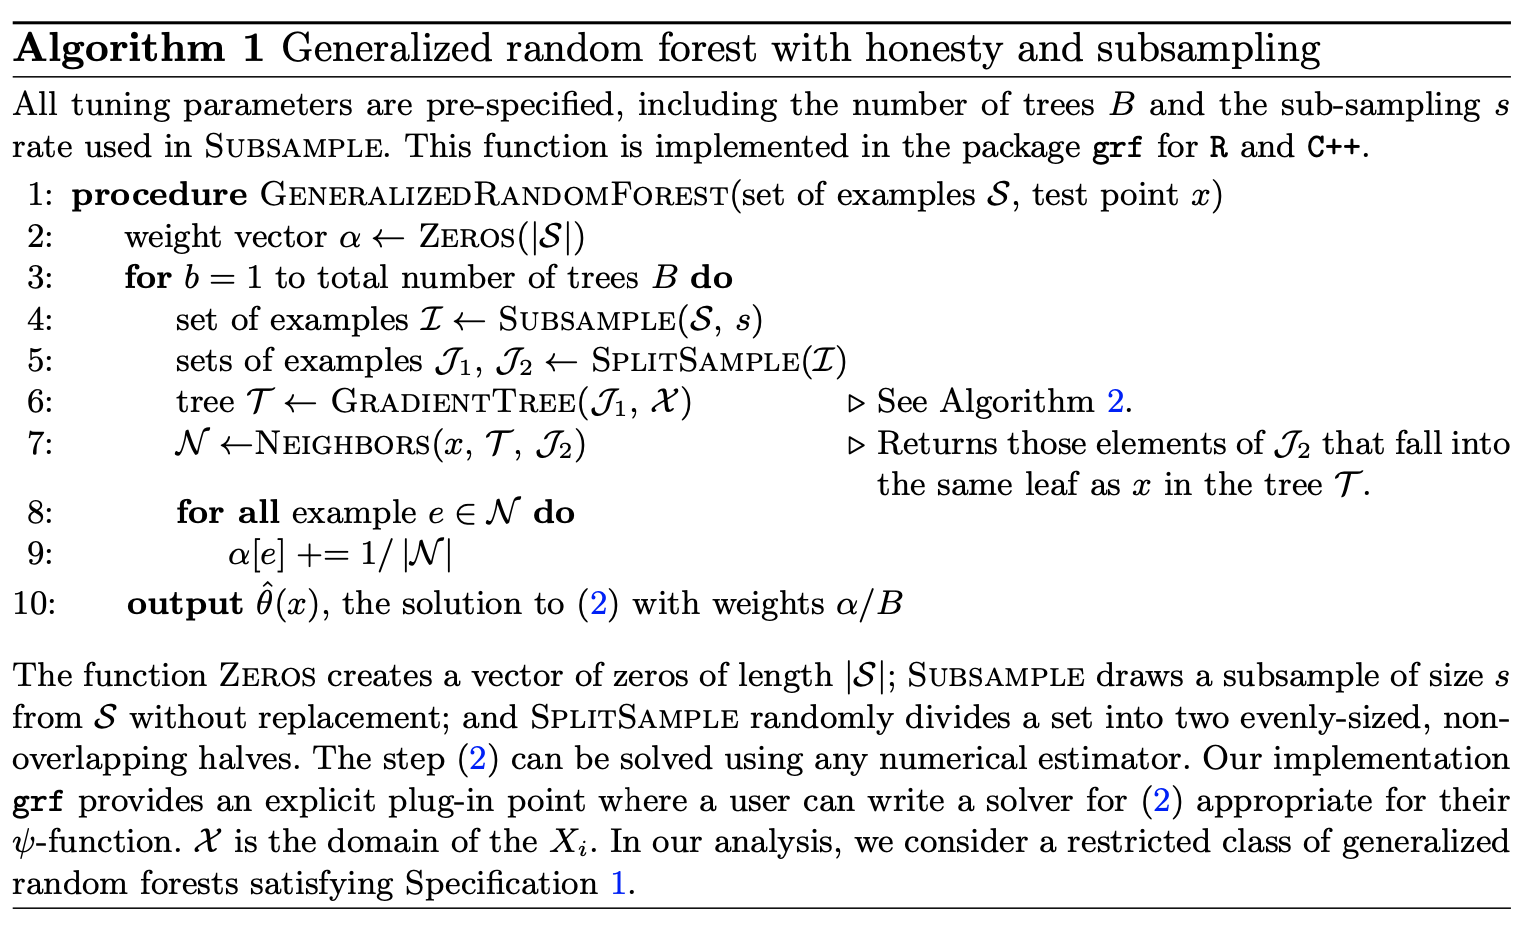
\includegraphics[width = 0.475\textwidth, height = 4.5cm]{Figures/grf/grfAlgo1.png}
	}
	\subfigure[Algorithm 2]{%
	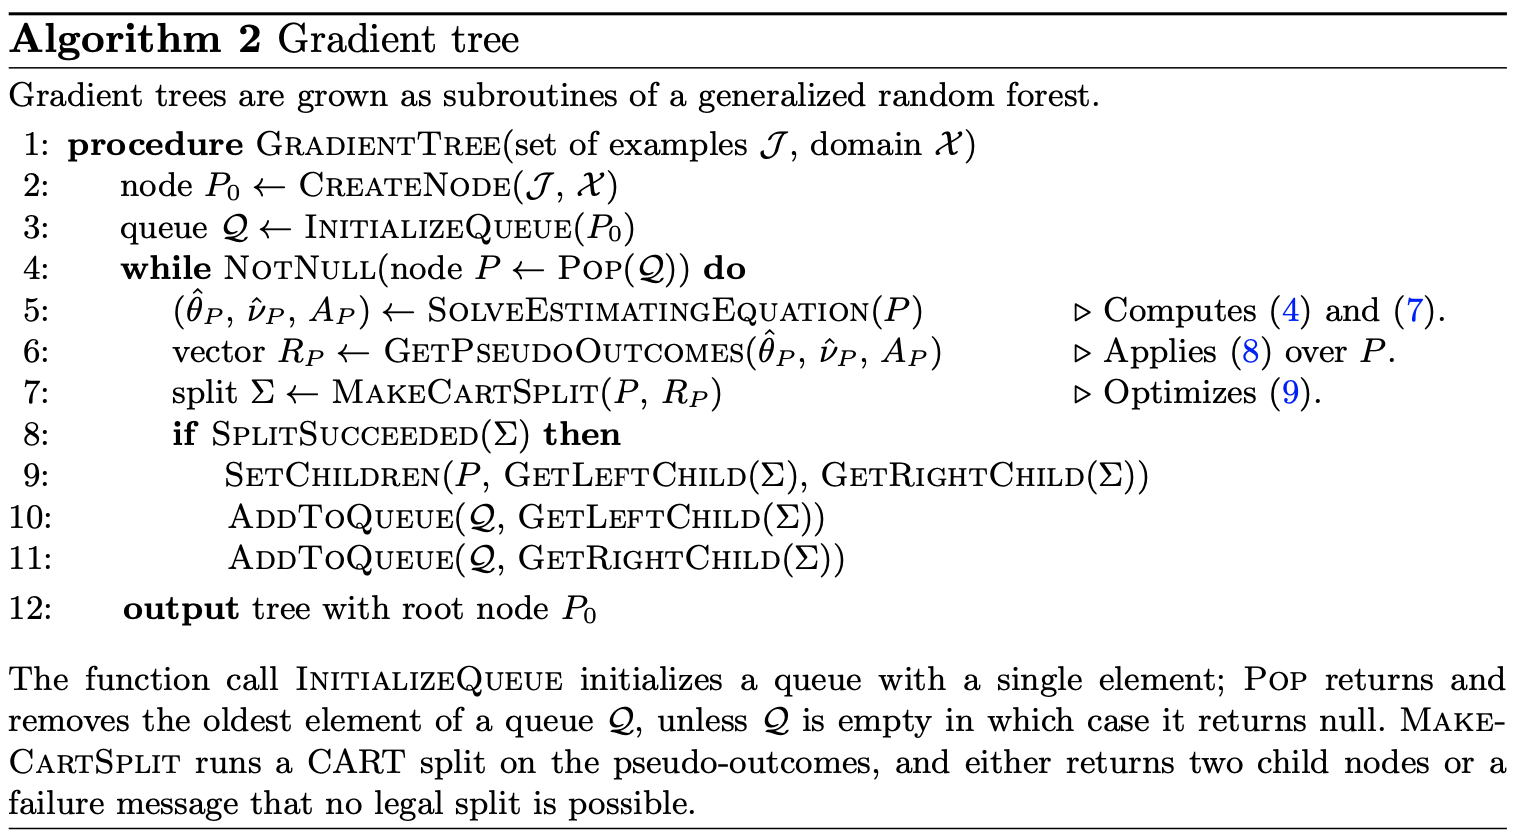
\includegraphics[width = 0.475\textwidth, height = 4.5cm]{Figures/grf/grfAlgo2.png}
	}
	\caption{Algorithms for growing generalized random forests}
\end{figure}

In contrast to using a regression splitting criterion as in \ref{eq:regression_step_criterion}, which only requres a single pass over the data in the parent node, directly optimizing the original criterion in eq. \ref{eq:delta_criterion} may require optimizing at every possible candidate split. This sort of gradient based approximation also underlies other popular statistical algorithms, including gradient boosting (Friedman, 2001) and model based recursive partitioning algorithm of Zeileis, Hothorn, and Hornik (2008).

Paper can verify that the error from using the approcimate criterion $\DeltaT$ instead of the exact $\Delta$-criterion is within the tolerance used to motivate the $\Delta$-criterion in Proposition $1$, thus suggesting that use of it may not result in too much ineffeciency. Consistent estimates of $A_P$ can, in general, be derived directly, without relying on the proposition below
\begin{prop}
Under the conditions of Proposition \ref{prop1}, if $|A_P - \nabla\mathbb{E}[\psi_{\thetaH_P, \nuH_P}(O_i)|X_i \in P]| \rightarrow_P 0$, then $\Delta(C_1, C_2)$ and $\DeltaT(C_1,C_2)$ are approximately equivalent in that 
\[\DeltaT(C_1,C_2) = \Delta(C_1,C_2) + o_P\left(\max\{r^2, 1/n_{C_1}, 1/n_{C_2}\}\right)\]
\end{prop}

Now, given a practical splitting scheme for growing individual trees, we want to grow a forest that allows for consistent estimation of $\theta(x)$ using \ref{eq:theta_nu_sample} using the forest weights in eq. \ref{eq:alpha_bi}. Each tree will provide small, relevant neighborhoods for $x$ that will lead to noisy estimates of $\theta(x)$; then we may hope that forest based aggregation will provide a single larger but still relevant neighborhood of $x$ that yields stable estimates $\thetaH(x)$. Rely on two conceptual ideas that have proven to be succesful in the literature on forest-based least-squares regression. 
Training trees on subsamples of the data nd a subsampling splitting technique called ``honesty''.

\subsection{Asymptotic Analysis}

Aim of this section is to establish asymptotic Gaussianity of the $\thetaH(x)$ and of providing tools for statistical inference about $\theta(x)$. The covariate space and the parameter space are both subsets of Euclidean space. Specifically $\mathscr{X} = [0,1]^p$ and $(\theta, \nu) \in \mathscr{B} \subset \mathbb{R}^k$ for some $p,k > 0$ and $\mathscr{B}$ is a compact subset.\footnote{This seems to restrict $\theta$ to be semiparametric. I don't think that is the right interpretation though. $\theta(x)$ can still be an arbitrary function taking values on a the real line.} Moreover, we assume that $X$ has a density that is bounded away from 0 and from above. This is a weaker requirement in the forest prediction space since trees and forests are invariant to monotone rescaling of the features.

Some practically interesting cases, such as quantile regression involve discontinuous score functions $\psi$, which complicates analysis. Here we assume that the spected score function
\begin{equation}
	\label{eq:expected_score}
	M_{\theta,\nu}(x) := \mathbb{E}[\psi_{\theta,\nu}(O)|X = x]
\end{equation}
varies smoothly in the parameters, even though $\psi$ itself may be discontinuous. For example, with quantile regression $\psi_{\theta}(Y) = \mathbf{1}(\{Y > \theta\}) - (1-q)$ is discontinuous in $q$ and $Y$, but $M_\theta(x) = \mathbb{P}[Y > \theta | X = x] - (1-q)$ is smooth whenever $Y|X=x$ has a smooth density. We add the following assumptions

\begin{assumption}{(Lipschitz $x$-signal) }
\label{as:lipschitz}
For fixed valued of $(\theta, \nu)$ we assume that $M_{\theta,\nu}(x)$ is Lipschitz continuous in $x$. 
\end{assumption}

\begin{assumption}{(Smooth identification) }
\label{as:smooth_id}
When $x$ is fixed, assume that the $M$-function is twice continuously differentiable in $(\theta, \nu)$ with a uniformly bounded second derivative, and that $V(x) := V_{\theta(x), \nu(x)}(x)$ is invertible for $x \in \mathscr{X}$, with $V_{\theta,\nu}(x) := \frac{\partial}{\partial(\theta, \nu)} M_{\theta,\nu}(x)\bigg|_{\theta(x),\nu(x)}$.
\end{assumption}
\begin{assumption}{(Lipschitz $(\theta, \nu)$-variogram) }
\label{as:lipschitz_variogram}
The score functions $\psi_{\theta,\nu}(O_i)$ have a continuous covariance structure. Writing $\gamma$ for the worst-case variogram and $\Vert \cdot \Vert_{F}$ for the Frobenius norm, then for some $L > 0$
\begin{align*}
\gamma\left( \begin{pmatrix} \theta \\ \nu \end{pmatrix}, \begin{pmatrix} \theta' \\ \nu' \end{pmatrix}    \right) &\leq L \left\Vert \begin{pmatrix} \theta \\ \nu \end{pmatrix} - \begin{pmatrix} \theta' \\ \nu' \end{pmatrix}  \right\Vert_2 \\
\gamma\left( \begin{pmatrix} \theta \\ \nu \end{pmatrix}, \begin{pmatrix} \theta' \\ \nu' \end{pmatrix}    \right) &:= \sup_{ x \in \mathscr{X} }\{\Vert \Var [\psi_{\theta, \nu}(O_i) - \psi_{\theta', \nu'}(O_i) | X_i = x]\Vert_F  \}
\end{align*}
\end{assumption}

\begin{assumption}{(Regularity of $\psi$) }
\label{as:psi_regularity}
The $\psi$-fucntions can be written as $\psi_{\theta, \nu}(O) = \lambda(\theta, \nu; O_i) + \zeta_{\theta, \nu}(g(O_i))$ such that $\lambda$ is Lipschitz-continuous in $\theta, \nu$ and $g: {O_i} \rightarrow \mathbb{R}$ is a univariate summary of $O_i$, and $\zeta_{\theta, \nu}: \mathbb{R} \rightarrow \mathbb{R}$ is any family of monotone and bounded functions
\end{assumption}
\begin{assumption}{(Existence of solutions) }
\label{as:existence}
We assume that, for any weights $\alpha_i$ with $\sum \alpha_i = 1$, the estimating equation returns a minimizer $(\thetaH, \nuH)$ that at least approximately solves the estimating equation: $\Vert \sum_{i=1}^n \alpha_i \psi_{\thetaH, \nuH}(O_i)\Vert_2 \leq C \max\{\alpha_i\}$ for some constant $C\geq 0$. 
\end{assumption}

\begin{assumption}{(Convexity) }
\label{as:convexity}
The score function $\psi_{\theta, \nu}(O_i)$ is a negative sub-gradient of a convex function, and the expected score $M_{\theta, \nu}(X_i)$ is the negative gradient of a strongly function. 
\end{assumption}
Assumption 3 holds trivially if $\psi$ is Lipschitz in the parameters. Assumption 4 is used to show that a certain empirical process is Donsker. The first 5 assumptions deal with local properties of the estimating equation and can be used to control the behavior of $(\thetaH(x), \nuH(x))$ in neighborhoods of the population parameter value $(\theta(x), \nu(x))$. The 6th assumption garuntees consistency. 

Consistency and Gaussianity results require using some specific settings for the trees from Algorithm 1. In particular, require that all trees are honest and regular in the sense of Wager and Athey (2018), as follows. In order to satisfy the minimum split probability condition below, our implementation relies on the device of Denil, Matheson and De Freitas (2014), whereby the number splitting variables considered at each step of the algorithm is random. Specifically, try $\min\{\max\{\Poisson(m), 1\},p\}$ variables at each step, where $m > 0$ is a tuning parameter.
\begin{specification}
All trees are symmetric in that their output is invariant to permuting the indices of training examples; make balanced splits in the sense that every split puts at least a fraction $\omega$ of the observations in the parent node into each child, for some $\omega > 0$; and are randomized in such a way that, at every split, the probability that the tree splits on the $j$-th feature. is bounded from below by $\pi > 0$. The forest is honest and built with subsample size satisfying $s/n \rightarrow 0$ and $s \rightarrow \infty$.
\end{specification}

These assumptions hold trivially under some weak assumptions for least squares and quantile regression.

\subsubsection{A Central Limit Theorem for Generalized Random Forests}

Now ready for asymptotic results. Note that regression forests are averages of regression trees grown over sub-samples and were thus be analyzed as $U$-statistics (Hoeffding, 1948). Unlike regression forest predictions, however, the parameter estimates $\thetaH(x)$ from generalized random forests are not averages of estimates made by different trees. Instead, we obtain $\thetaH$ by solving a single weighted moment equation as in eq. \ref{eq:mc_sample}. So existing proof strategies do not apply in thi setting. 

Tackle this problem using method of influence functions as described by Hampel (1974). In particular, we are motivated by the analysis of Newey (1994a). Core idea is to derive a sharp, linearized approzimation to the local estimatior, and then to analyze the linear approximation instead. Let $\ris(x)$ denote the influence function on the $i$-th observation with respect to the true parameter value, $\theta(x)$
\[\ris(x) := -\xi^TV(x)^{-1}\psi_{\theta(x),\nu(x)}(O_i)\]
Then, given any set of forest weights $\alpha_i(x)$ used to define the generalized random forest estimate $\thetaH(x)$ by solving (\ref{eq:mc_sample}) define a pseudo-forest 
\begin{equation}
\label{eq:thetaHat_appx}
	\thetaT^*(x) := \theta(x) + \sum_{i=1}^n \alpha_i(x) \ris(x)
\end{equation}
used to approximate $\thetaH(x)$. $\thetaT^*(x)$ is the output of an infeasible regression forest with weights $\alpha_i(x)$ and outcomes $\theta(x) + \ris(x)$. The upshot is that this is a $U$-statistic, which we know how to analyze. Because $\thetaT^*(x)$ is a linear function of the pseudo outcomes $\ris(x)$, it can be written as an average of pseudo-tree predictions $\thetaT^*(x) = \frac{1}{B}\sum_{b=1}^B \thetaT_{b^*}(x)$ where $\thetaT_{b^*}(x) = \sum_{i=1}^n \alpha_{ib}(x)(\theta(x)+ \ris(x))$. Then, because each individual pseudo-tree prediction $\thetaT_{b^*}$ is trained on a size $s$ usbsample of the training data, drawn without replacement, $\thetaT^*(x)$ is an infinite order $U$-statistic whose order corresponds to the subsample size. 
\begin{itemize}
	\item Arguments of Mentch and Hooker (2016) and Wager and Athey (2018) can be used to study the averaged estimator $\thetaT^*(x)$ using results on U-statistics from Hoeffding (1948) and Efron and Stein (1981)\footnote{The definition of U-statistic from Hoeffding (1948), via Wikipedia. Let $f: \mathbb{R}^r \rightarrow \mathbb{R}$ be a real-valued or complex-valued function of $r$ variables. For each $n\geq r$, the associated $U$-statistic $f_n:\mathbb{R}^n \rightarrow \mathbb{R}$ is equal to the average over ordered samples $\varphi(1), \dots, \varphi(r)$ or size $r$ of the sample values $f(x_\varphi)$. In otherwords $f_n(x_1, \dots, x_n) = \text{ave} f(x_{\varphi(1), \dots, x_\varphi(r)})$. By neccesity, each U-statistic is a symmetric function.} 
\end{itemize}
Difficulty in this proof stratefy is showing that $\thetaT^*(x)$ is a good approximation for $\thetaT(x)$. Following theorem establishes this. This is the only point where $\phi$ being the negative gradient of a convex loss function is used. 
\begin{theorem}
	\label{thm:consistency}
	Under Assumptions 1-6, estumatees $\thetaH(x), \nuH(x)$ converge in probability to $\theta(x), \nu(x)$.
\end{theorem}
Seperating the analysis of moment estimators into a local approcumation argument that hinges on consistency and a seperate result that estabilishes consistency is standard; see chapter 5.3 of Van Der Vaart (2000)\footnote{Textbook is \textit{Asymptotic Statistics} and it can be found in the google drive}

The remainder of analysis assumes that trees are grown on subsamples of size $s$ scalig as $s = n^\beta$ for some $\beta_{\min} < \beta < 1$ with 
\begin{equation}
	\label{eq:betaMin}
	\beta_{\min} := 1 - \left(1 + \pi^{-1}\left(\log(\omega^{-1})\right)\right)^{-1}
\end{equation}
where $\pi$ and $\omega$ are as in Specification 1. Scaling garuntees errors of forests are varaicne-dominated. 

\begin{lemma}
\label{thm:main-result}
Given Assumptions 1-5 and a forest trained according to Specification 1 with condition \ref{eq:betaMin} holding, suppose that the generalized random forest estimator $\thetaH$ is consistent for $\theta(x)$. Then $\thetaH(x)$ and $\thetaT^*(x)$ are coupled at the following rate
\begin{equation}
	\sqrt{\frac{n}{s}}\left(\theta^*(x) - \thetaH(x)\right) = \mathscr{O}_P \left( \max\left\{ 
	s^{-\frac{\pi \log \left( (1-\omega)^{-1}\right)}{2 \log \left( \omega^{-1}\right)}}, \left(\frac{s}{n}\right)^{\frac{1}{6}}\right\} \right)
\end{equation}
where $s$, $\omega$ and $\pi$ are as in Specification 1.
\end{lemma}
Given this coupling result, it now remains to study the asymptotics of $\thetaT^*(x)$. In doing so, important to know that $\thetaT^*(x)$ is exactly the output of an infeasible regression forest trained on outcomes $\theta(x) + \ris(x)$. So can apply results of Wager and Athey (2018) to this object. With this approach, authors show that, given \ref{eq:betaMin}m $\thetaT^*(x)$ and $\thetaH(x)$ are both asymptotically normal. Extending the argument can also so this for nuisance parameters, but noting that since tree is not trained to optimize nuisance, may not work well in finite samples. 
\begin{theorem}
	\label{thm:clt}
	Suppose Assumptions 1-6 hold and a forest is trained according to Specification 1 with trees grown on subsamples of size $s = n^\beta$ satisfying \ref{eq:betaMin}. Finally, suppose that $\Var[\ris(x)|X=x] > 0.$ Then, there is a sequence $\sigma_n(x)$ for which $(\thetaH_n(x) - \theta(x))/\sigma_n(x) \rightarrow \mathscr{N}(0,1)$ and $\sigma_n^2(x) = \polylog(n/s)^{-1}s/n$, where $\polylog(n/s)$ is a function that is bounded away from 0 and increases at most polynomially with the log-inverse sampling ratio $\log(n/s)$. 
\end{theorem}
\subsection{Confidence Intervals via the Delta Method}
Theorem \ref{thm:clt} can be used for statistical inference about $\theta(x)$. Given a consistent estimator $\hat{\sigma}_n(x)$ for $\sigma_n(x)$, Theorem \ref{thm:clt} can be paired with Sltutsky's lemma to verify
\[\lim_{n\rightarrow\infty} \mathbb{P}\left[\theta(x) \in \left(\thetaH(x) \pm \Psi^{-1}(1-\alpha/2)\hat{\sigma}_n(x)\right)\right] = \alpha\]
So to build asymptotically valid pointwise confidence intervales, it suffices to derive an estimator for $\sigma_n(x)$. Doing so requires leveraging coupling with the approximate pseudo-forest $\thetaT^*(x)$. Moreover, from the definition of $\thetaT^*(x)$, we directly see that 
\begin{equation}
	\label{eq:varThetaT*}
	\Var\left[\thetaT^*(x)\right] = \xi^T V(x)^{-1} H_n\left(x; \theta(x), \nu(x)\right)\left(V(x)^{-1}\right)^T \xi
\end{equation}
where $H_n(x;\theta, \nu) = \Var[\sum_{i=1}^n \alpha_i(x) \psi_{\theta,\nu}(O_i)]$. Authors then propose building confidence intervals via
\begin{equation}
	\label{eq:sigmaHat}
	\hat{\sigma}_n^2 := \xi^T \hat{V}_n(x)^{-1} \hat{H}_n(x) (\hat{V}_n(x)^{-1})^T \xi
\end{equation}
Coming up with consistent estimators of $V(x)$ is well studied and not so complex, according to the authors. Estimating $H$, however, can be difficult since it depends on the true forest score $\Psi(\theta(x), \nu(x)) = \sum_{i=1}^n \alpha_i(x) \psi_{\theta(x), \nu(x)}(O_i)$. To estimate this, they use a variant of the bootstrap of little bags algorithm (noisy bootstrap) proposed by Sexton and Laake (2009). They obtain the first consitency garuntees for this method for any type of forest, including regression forests. Notes about this are breifly given below

\subsubsection{Consistency of the Bootstrap of Little Bags}



\newpage
%!TEX root = /Users/manunavjeevan/Desktop/Research/ML + Lasso/Annotated Literature Review/litNotesML.tex

\section{Deep Learning in NPR \textit{\small Benedikt Bauer and Michael Kohler (AOS, 2019)}}
\label{sec:dl_npr}
Full paper title is ``On Deep Learning As A Remedy for the Curse of Dimensionality in Nonparametric Regression'' and can be found via the AoS website 
\href{https://projecteuclid.org/download/pdfview_1/euclid.aos/1558425645}{here}.

\subsection{Introduction}

In regression analysis, a random vector $(X,Y)$ with values in $\mathbb{R}^d \times \mathbb{R}$ satisfying $\mathbf{E}Y^2 < \infty$ is considered, and an estimation of the relationship between $X$ and $Y$ is attempted. Generally the aim is to minimize the MSE or $L_2$r risk. So the construction of a measurable function $m^*: \mathbb{R}^d \rightarrow \mathbb{R}$ satisfying 
\[m^* =\argmin_{f: \mathbb{R}^d \rightarrow \mathbb{R}} \mathbf{E}\left\{\left|Y- f(X)\right|^2\right\}\]
is of interest. In the following, let $m:\mathbb{R}^d \rightarrow \mathbb{R}$, $m(x) = \mathbf{E}\{Y|X=x\}$ denote the ``regression function''. It is true that for any $f$:
\[\mathbf{E}\left[ \left|Y-f(X)\right|^2\right] = \mathbf{E}\left[\left|Y - m(X)\right|^2\right] + \int \left| f(x) - m(x) \right|^2 \mathbf{P}_X(dx) \]
it is the optimal predictor $m^*$. Moreover, a good estimate $f:\mathbb{R}^d \rightarrow \mathbb{R}$ (in the $L_2$ risk minimization sense) has to keep the ``$L_2$'' error small 
\[\int \left|f(x) - m(x)\right|^2 \mathbf{P}_X(dx)\]
In applications, the distribution of $(X,Y)$ and $m$ are (typically) unkown, but the statistician does have access to a set of data 
\[\mathscr{D}_n = \{(X_1,Y_1), \dots, (X_n, Y_n)\}\]
Goal is typically to create estimates of $m$, $m_n$ to minimize the $L_2$ error. In non-parametric regression estimation of the regression function does not reduce to estimation of finitely many parameters. Gyordi et al. (2002) provide a systematic overview of different approaches and nonparametric estimation results.

\subsubsection{Rate of Convergence}
Well known that one has to restric the class of regression functions one considers to obtain useful results for the rate of convergence. Following definiton of $(p,C)$-smoothness is to that end
\begin{definition}
\label{def:DLNPR-1}
($(p,C)$-smooth) Let $p = q + s$ for some $q \in \mathbb{N}_0$ and $0 < s \leq 1$. A function $m:\mathbb{R}^d \rightarrow \mathbb{R}$ is called $(p,C)$-smooth if, for every $\alpha = (\alpha, \dots, \alpha_d) \in \mathbb{N}_0^d$ with $\sum_{j=1}^d \alpha_j = q$, the partial derivatives below exist and satisfy
 \[\left|\frac{\partial^q m }{\partial x_1^{\alpha_1} \cdots \partial x_d^{\alpha_d}}(x) - \frac{\partial^q m }{\partial x_1^{\alpha_1} \cdots \partial x_d^{\alpha_d}}(z)  \right| \leq C \Vert x-z\Vert^s \]
 for all $x,z \in \mathbb{R}^d$, where $\Vert \cdot \Vert$ denotes the Euclidean norm.\footnote{This is similar to the Holder condition we went over with Zhipeng}
\end{definition}
 Stone (1982) determined the optimal minimax rate of convergence in nonparametric regresion for $(p,C)$-smooth functions. A sequence of eventually positive numbers $(a_n)_{n\in\mathbb{N}}$ is called a \textit{lower minimax rate of convergence} for the class of distributions $\mathscr{D}$ if 
 \[\liminf_{n\rightarrow\infty} \inf_{m_n} \sup_{(X,Y)\in \mathscr{D}} \frac{\mathbf{E}\int |m_n(x) - m(x)|^2 \mathbf{P}_X(dx)}{a_n} = C_1 > 0\]
Sequence is said to be an \textit{achievable rate of convergence} for the class of distributions $\mathscr{D}$ if 
\[\limsup_{n\rightarrow\infty}\sup_{(X,Y)\in \mathscr{D}}\frac{\mathbf{E}\int |m_n(x) - m(x)|^2 \mathbf{P}_X(dx)}{a_n} = C_2 > 0\footnote{Achievable in the sense that it is the minimax rate of convergence for at least one estimator $m_n$} \]

Sequence is called an \textit{optimal minimax rate of convergence} if it both a lower minimiax and achievable rate of convergence. Stone (1982) shows that the optimal rate of convergence for the estimation of a $(p,C)$-smooth regression function is $n^{-\frac{2p}{2p+d}}$

\subsubsection{Curse of dimensionality}
Optimal rate $n^{-\frac{2p}{2p+d}}$ suffers if $d$ is relatively large compared with $p$. Phenomenon is well known and called the curse of dimensionality. Unfortunately, in many applications, the problems are high dimensional and hence very hard to solve. Only way around this is to impose additional assumptions on the regression function to derive better rates of convergence. For example, under additive seperability of the regression function, Stone (1985) shows that the optimal minimax rate of convergence is $n^{-2p/(2p+1)}$.

Paper focuses on applications in connection with complex technical systems, constructed in a modular form. In this case, modeling the outcome of the system as a function of the results of its modular parts seems reasonable, where each modular part computes a function depending only on a few of the components of the high-dimensional input. Modularity can be extremely complex and deep. So, a recursive application of the described relation makes sense and leads to the following assumption of $m$, introduced by Kohler and Kryzak (2017). 

\begin{definition}
	\label{def:DLNPR-2}
	Let $d\in\mathbb{N}, d^* \in \{1, \dots, d\}$ and $m:\mathbb{R}^d \rightarrow \mathbb{R}$. Then:
	\begin{enumerate}
		\item We say that $m$ satisfies a \textit{generalized hierarchical interaction of order $d^*$ and level 0} if there exist $a_1,\dots a_{d^*} \in \mathbb{R}^d$ and $f:    \mathbb{R}^d \rightarrow \mathbb{R}$ such that 
		\[m(x) = f(a_1^T x, \dots, a_{d^*}^T x)\hbox{ }\hbox{ }\text{ for all $x \in \mathbb{R}^d$}\]
		\item We say that $m$ satisfies a \textit{generalized hierarchical model of order $d^*$ and level $l+1$}, if there exist $K \in \mathbb{N}, g_k:\mathbb{R}^{d^*} \rightarrow \mathbb{R}$ for $k = 1, \dots, K$, and $f_{1,k}, \dots, f_{d^*,k}: \mathbb{R}\rightarrow \mathbb{R}$ for $k = 1,\dots, K$ such that all $f_{1,k},\dots,f_{d^*,k}$ satisfy a generalized hierarchical interaction model of order $d^*$ at level $l$ and 
		\[m(x) = \sum_{k=1}^K g_k\left(f_{1,k}(x),\dots,f_{d^*,k}(x)\right)\hbox{ }\hbox{ }\text{ for all $x \in \mathbb{R}^d$}\]
		\item We say that the $\textit{generalized hierarchical interaction model}$ defined above is $(p,C)$-smooth if all functions occuring in its definition are $(p,C)$-smooth.
	\end{enumerate}
\end{definition}

To better understand the above definition, we consider the additive model from the beggining of this section as an example. Notate $\id:\mathbb{R}\rightarrow\mathbb{R}$ for the identity function and $e_i$ for the $i$th unit vector. Can then rewrite the additive model as 
\[\sum_{i=1}^d m_i(x^{(i)}) = \sum_{i=1}^d m_i(\id(e_i^Tx)) = \sum_{i=1}^K g_i(f_{1,i}(a_i^Tx))\]
where $K = d, g_i = m_i, f_{1,i} = \id$ and $a_i = e_i$. This corresponds to the definition of a gneralized hierarchichal interaction model of order 1 and level 1. 

\subsubsection{Neural Networks}
Use of neural networks has been most promising approaches in connection with applications related to approxumation and estimation of multivariate functions. Recently, focus is on multilayer neural networks, which use many hidden layers and corresponding techniques.

Multilayer feedforward neural networks with a sigmoidal function $\sigma: \SR\rightarrow [0,1]$ can be defined recursively as follows. A multilayer feedforward neural network with $l$ hidden layers, which has $K_1, \dots, K_l \in \SN$ neurons in the first, second, through $l$-th layer, respectively, and uses the activation function $\sigma$ is a real valued function defined on $\SR^d$ of the form 
\begin{equation}
	\label{eq:DLNPR-1}
	f(x) = \sum_{i=1}^{K_l} c_i^{(l)}\cdot f_i^{(l)} + c_0^{(l)}, \footnote{We can think about this as a linear regression of the outcome against equations from the final layer}
\end{equation}
for some $c_0^{(l)}, \dots, c_{K_l}^{(l)}\in \SR$ and for $f_i^{(l)}$ recursively defined by
\begin{equation}
	\label{eq:DLNPR-2}
	f_i^{(r)}(x) = \sigma\left(\sum_{j=1}^{K_{r-1}} c_{i,j}^{(r-1)} \cdot f_j^{(r-1)}(x) + c_{i,0}^{(r-1)}\right), \footnote{Apply a sigmoid function to a linear combination of the outputs from the prior round. To clarify some notation:  $f_j^{(r-1)}$ is the output from the $j$-th neuron in the $(r-1)$-th layer, $c_{i,j}^{(r-1)}$ is the weight given at neuron $i$ in the $r$-th layer to the output of the $j$-th neuron in the $(r-1)$-th layer. There are $K_r$ neurons at each layer $r$, so that each neuron in layer $r$ has to ``pick'' appropriate weights for all $K_{r-1}$ outputs of neurons in layer $(r-1)$.}
\end{equation}
for some $c_{i,0}^{(r-1)}, \dots, c_{i,K_{r-1}}^{(r-1)} \in \SR$ and $r = 1, \dots, l$ and 
\begin{equation}
	\label{eq:DLNPR-3}
	f_i^{(1)}(x) =  \sigma\left(\sum_{j=1}^{d} c_{i,j}^{(0)} \cdot x^{(j)} + c_{i,0}^{(0)}\right), \footnote{$x^{(j)}$ is the $j$-th ``feature'', ``variable'', ``column'', what have you.}
\end{equation}
for some $c_{i,0}^{(0)}, \dots, c_{i,d}^{(0)}\in \SR$. Neural network estimates often use an activation function $\sigma: \SR\rightarrow[0,1]$ that is nondecreasing and satisfies 
\[\lim_{z\rightarrow-\infty} \sigma(z) = 0\hbox{ }\text{ and }\hbox{ }\lim_{z\rightarrow\infty} \sigma(z) = 1\]
for example, the so-called sigmoidal or logistic squasher 
\[\sigma(z) = \frac{1}{1 + \exp(-z)}, \forall z \in \SR\]
Most existing theoretical results concerining neural networks consider neural networks using only one hidden layer, that is functions of the form 
\begin{equation}
	\label{eq:DLNPR-4}
	f(x) = \sum_{j=1}^K c_j \cdot \sigma\left(\sum_{k=1}^d c_{j,k}\cdot x^{(k)} + c_{j,0}\right) + c_0
\end{equation}
Consistency of neural network regression estimates is studied by Meilnichzuk and Tyrcha (1993) and Lugosi and Zeger (1995). The rate of convergence has been analyzed by Barron (1991, 1993, 1993), McCaffery and Gallant (1994) and Kohler and Krzyzak (2005, 2017). For the $L_2$ error of a single hidden layer neural network, Barron (1994) proves a dimensionless rate of $n^{-1/2}$, provided the Fourier transform has a finite first moment. McCaffery and Gallant (1994) show a rate of $n^{-\frac{2p}{2p + d + 5} + \eps}$ for the $L_2$ error of a suitably defined single hidden layer neural network estimate for $(p,C)$-smooth functions, but their study was restricted to the use of a certain cosine squasher as the activation function.

Kohler and Krzyzak (2017) extends convergence results to $(p,C)$-smooth generalized hierarchical interaction models of the order $d^*$. It is shown that for such models suitable defined multilayer neural networks achieve the rate of convergence $n^{-2p/(2p+d^*)}$ in case $p\leq 1$. Nevertheless this result cannot generate extremely good rates of convergenve because, even in case of $p=1$ and $d^* = 5$, it leads to $n^{-2/7}$.

Given the succeful application of multilayer feedforward neural networks, the current focus in the theoretical analysis of approximation properties of neural networks is also on a a possible theoretical advantage of multilayer feedforward neural networks in contrast to neural networks with only one hidden layer. 

\subsubsection{Main Results}

This article analyzes the rate of convergence of suitable multilayer neural network regression estimates when the regression function satisfies a $(p,C)$-smooth generalized hierarchical interaction model of order $d^*$ and given level $l$. Unlike Kohler and Kryzak (2005, 2017) also allow the case $p > 1$, this leads to far better rates of convergence. Define sets of multilayer feedforward nueral netwroks that correspond to such a generalized a generalized hierarchical interaction model and define our regression estimates based on this class of neural networks. Main finding is that the $L_2$ errors of these least squares neural network regression estimates achieve the rate of convergence 
\[n^{-\frac{2p}{2p + d^*}}\]
up to some logarithmic factor which does not depend on $d$. Similar rates have been obrained in the literature but with much more stringent assumptions on the functional class the regression function belongs too. So this article considerably generalizes the previos results in this regard.

After the original versin of this paper, a relating arXiv article was uploaded by Schmidt-Heiber (2017). Therein a similar result is proven using a particular unbounded activation function in the neural networks    \href{https://arxiv.org/abs/1708.06633v2}{Available Here}

\subsubsection{Notation}

Let $A\subset \SR^d$ and $\calF$ be a set of functions $f:\SR^d\rightarrow \SR$ and let $\eps > 0$. A finite collection $f_1, \dots, f_N$ is called an $\eps$-$\Vert\cdot\Vert_{\infty, A}$-cover of $\calF$ if for any $f \in \calF$ there exists $i\in \{1, \dots, N\}$ such that 
\[\Vert f - f_i \Vert_{\infty, A} = \sup_{x\in A} |f(x) - f_i(x)| < \eps \]
The $\eps$-$\Vert\cdot\Vert_{\infty, A}$-covering number of $\calF$ is the size $N$ of the smallest $\eps$-$\Vert\cdot\Vert_{\infty, A}$-cover of $\calF$ and is denoted by $\calN(\eps, \calF,\eps$-$\Vert\cdot\Vert_{\infty, A})$\footnote{These are covered in Van derVaart and are important in the Donsker Theorems.}.


\subsection{Nonparametric Regression Estimation by Multilayer Feedforward Neural Networks}

Motivated by the generalized hierarchical interaction models, define spaces of hierarchical neural networks with parameters $K, M^*, D^*, d$ and level $l$ as follows. Parameter $M^*$ is introduced for technical reasons and originates from the composition of several smaller networks in the later proof of approximation results. $M^*$ controls the accuracy of the approximation and the ideal value will depend on certain properties of the estimated function. For $M^* \in \mathbb{N}, d \in \mathbb{N}, d^* \in [d]$ and $\alpha > 0$, denote the set of all functions $f: \mathbb{R}^d \rightarrow \mathbb{R}$ that satisfy
\[f(x) = \sum_{i=1}^{M^*} \mu_i \cdot \sigma \left(\sum_{j=1}^{4d^*}\lambda_{i,j}\cdot \sigma \left(\sum_{v = 1}^d \theta_{i,j,v}\cdot x^{(v)} + \theta_{i,j,0} \right) + \lambda_{i,0}\right) + \mu_0 \]
for $x\in \mathbb{R}^d$ and some $\mu_i, \lambda_{i,j}, \theta_{i,j,v}\in\mathbb{R}$ where 
\[|\mu_i|\leq \alpha, \hbox{ }|\lambda_{i,j}|\leq \alpha, \hbox{ }|\theta_{i,j,v}|\leq \alpha \]
for all $i \in \{0,1,\dots,M^*\}, j \in \{0,\dots, 4d^*\}, v\in{0,\dots,d}$ by $\calF_{M^*,d^*,d,\alpha}^{\text{(neural networks)}}$
In the first and second hidden layer, we use $4\cdot d^* \cdot M^*$ and $M^*$ neurons respectively. However, the neural network has only 
\begin{align*}
	\label{eq;DLNPR-5}
	W(\calF_{M^*,d^*,d,\alpha}^{\text{(neural networks)}}) &= M^* + 1 + M^*\cdot (4d^* + 1) + M^*\cdot4d^* \cdot(d+1) \\
	&= M^*\cdot(4d^* \cdot(d+2)+2) + 1\numberthis \\
\end{align*}
weights because the first and second hidden layer of the neural network are not fully connected. Instead, each neuron in te second hidden layer is connected with $4d^*$ neurons in the first hidden layer, and this is done in such a way that each neuron in the first hidden layer is connected with exactly one neural network in the second hidden layer. This is illustrated below in Figure \ref{fig:DLNPR-1}.
\begin{figure}[htbp!]
	\centering
	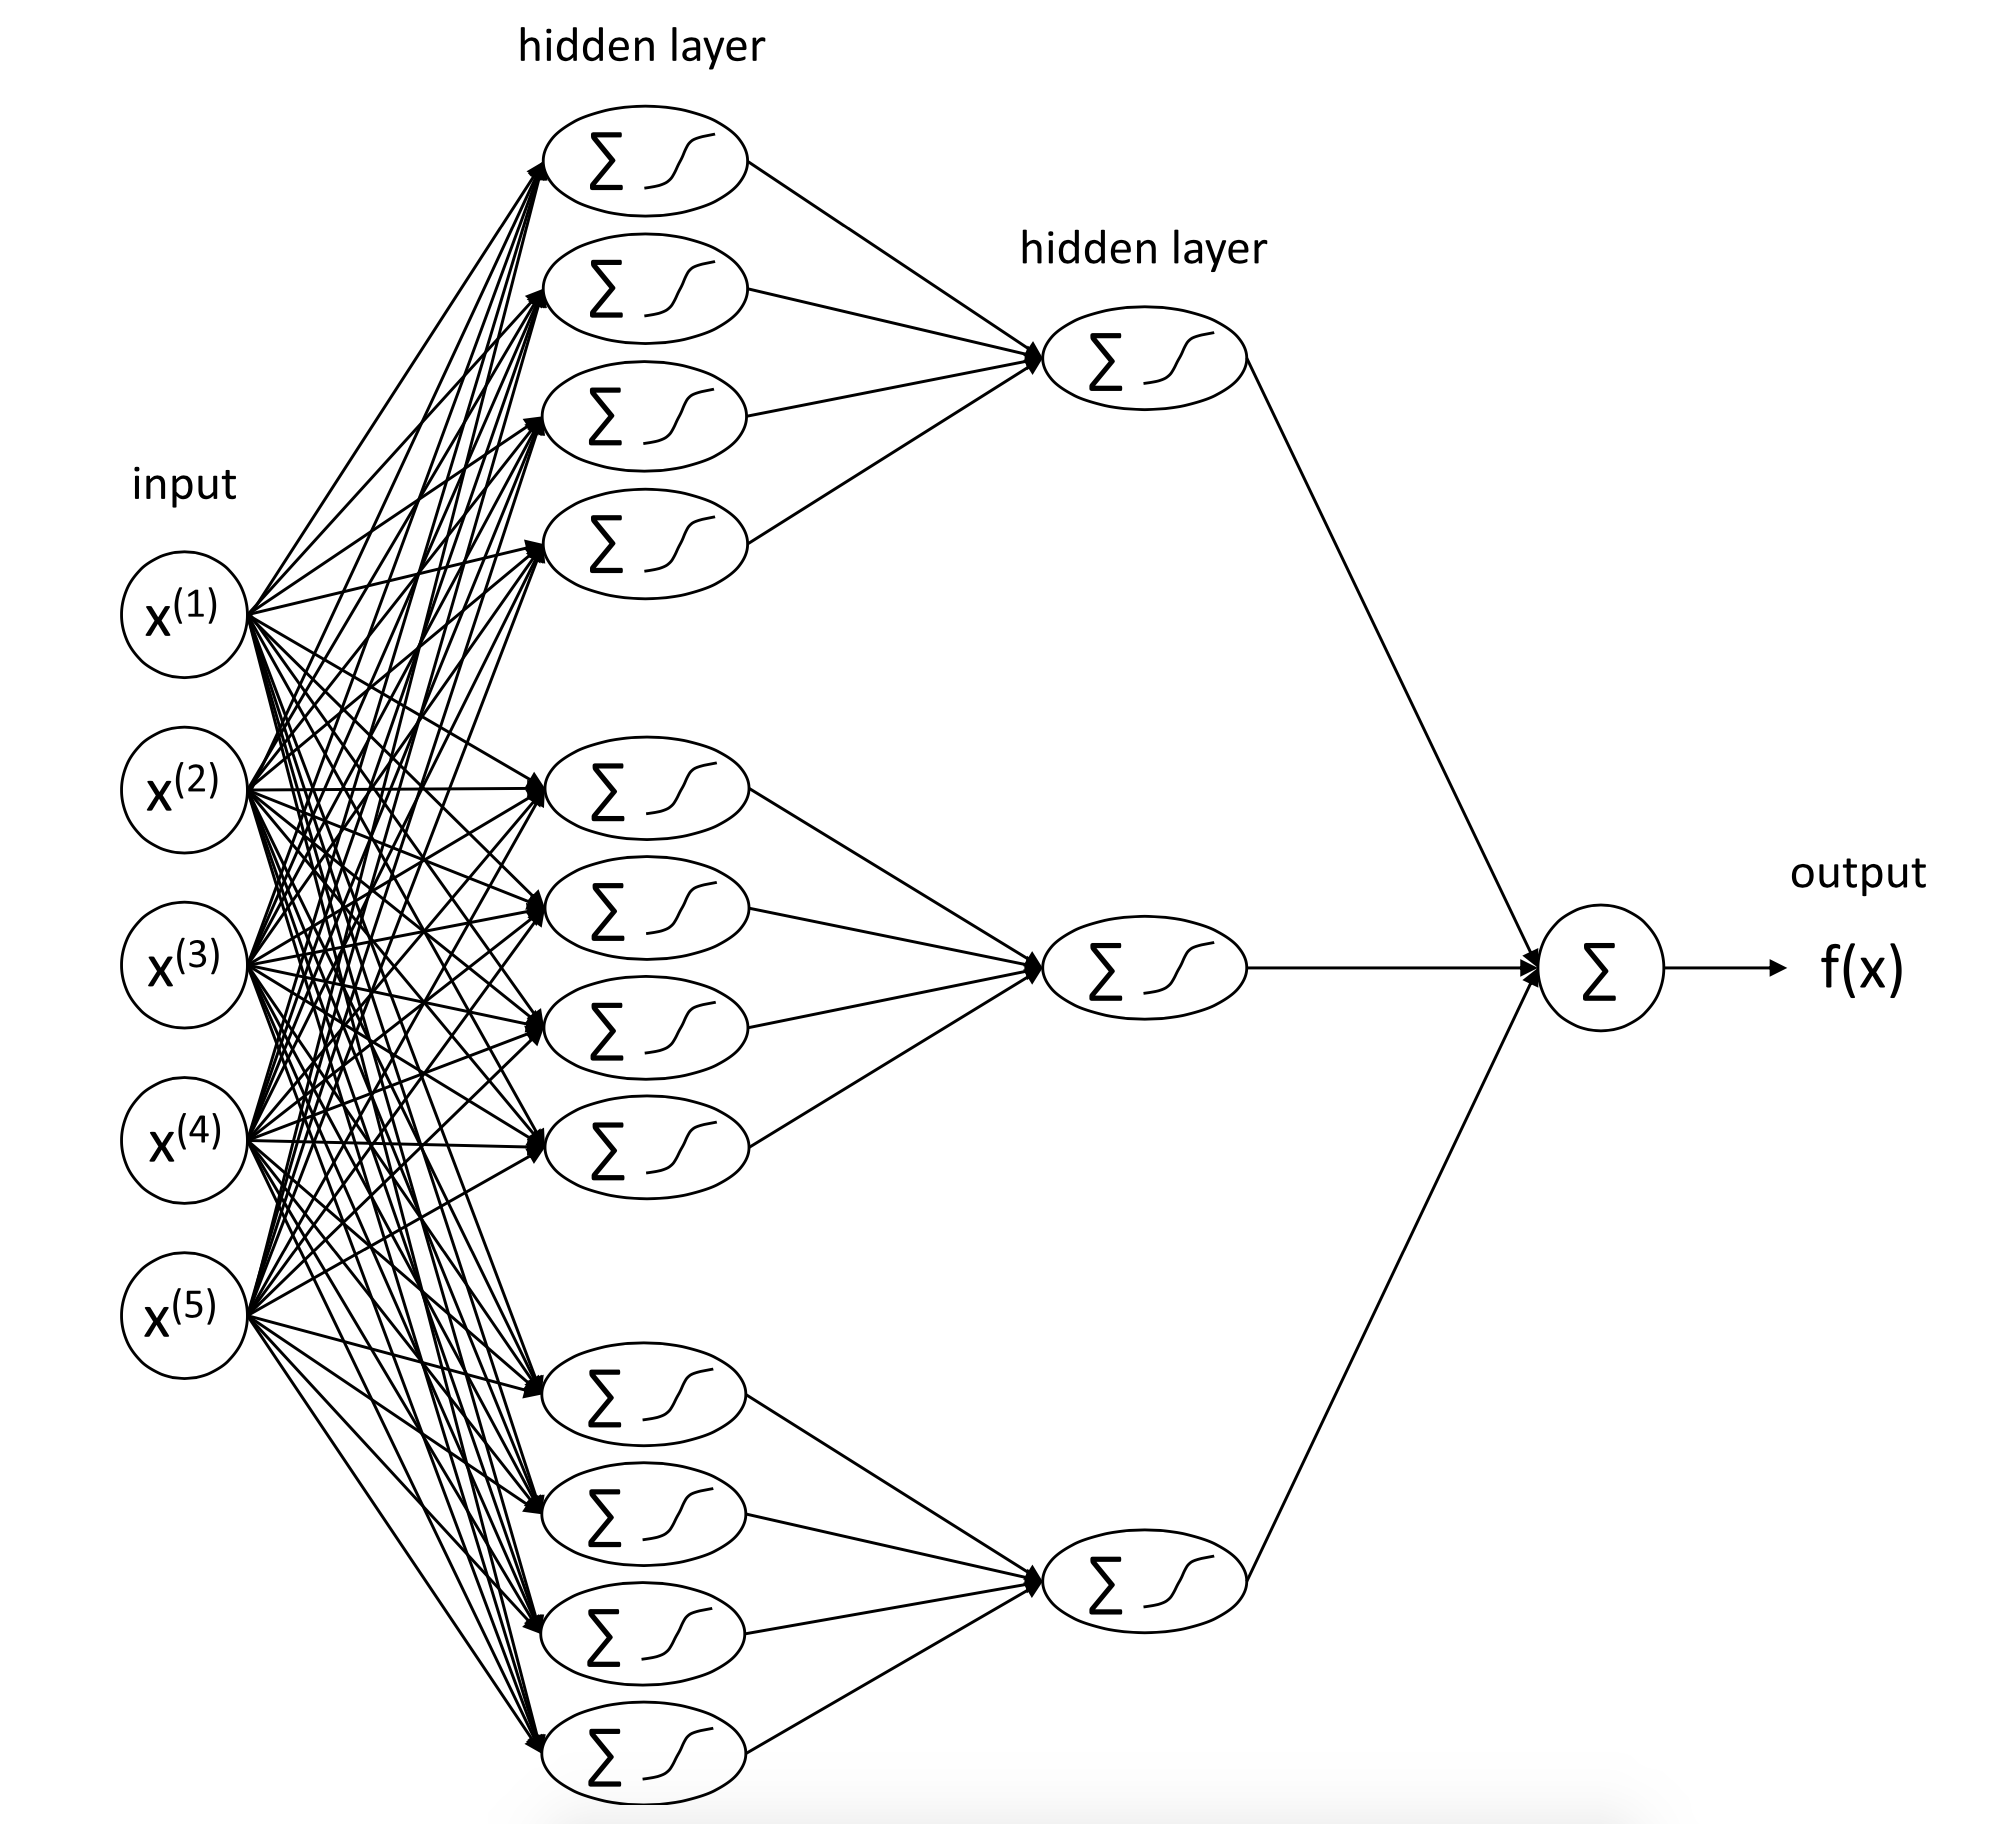
\includegraphics[width=0.75\textwidth]{Figures/DLNPR-Fig1}
	\caption{A not completely connected neural network $f:\SR^5\rightarrow \SR$ from $\calF_{M^*,d^*,d,\alpha}^{\text{(neural networks)}}$ with the structure $f(x) = \sum_{i=1}^3 \mu_i \cdot\sigma(\sum_{j=1}^4 \lambda_{i,j}\cdot\sigma(\sum_{v=1}^5 \theta_{i,j,v} \cdot x^{(v)}))$ (all weights with an index including zero neglected for a clear illustration). [Lifted from the paper]}
	\label{fig:DLNPR-1}
\end{figure}

For $l=0$, we define our space of hierarchical neural networks by 
\[\calH^{(0)} = \calF^{\text{(neural networks)}}_{M^*,d^*, d, \alpha} \]
For $l> 0$ we define recursively 
\begin{equation}
	\label{eq:DLNPR-6}
	\calH^{(l)} = \left\{h:\SR^d\rightarrow\SR: h(x) = \sum_{k=1}^K g_k(f_{1,k}(x),\dots, f_{d^*,k}(x))\text{ for some } g_k \in \calH^{(0)}\text{ and }f_{j,k} \in \calH^{(l-1)}\right\}
\end{equation}
The class $\calH^{(0)}$ is a set of neural networks with two hidden layers and a number of weights given by (\ref{eq;DLNPR-5}). From this, one can recursively conclude that for $l>0$, the class $\calH^{(l)}$ is a set of neural networks with $2\cdot l + 2$ hidden layers. This is illustrated below in Figure \ref{fig:DLNPR-Fig2}
\begin{figure}[htbp!]
	\centering
	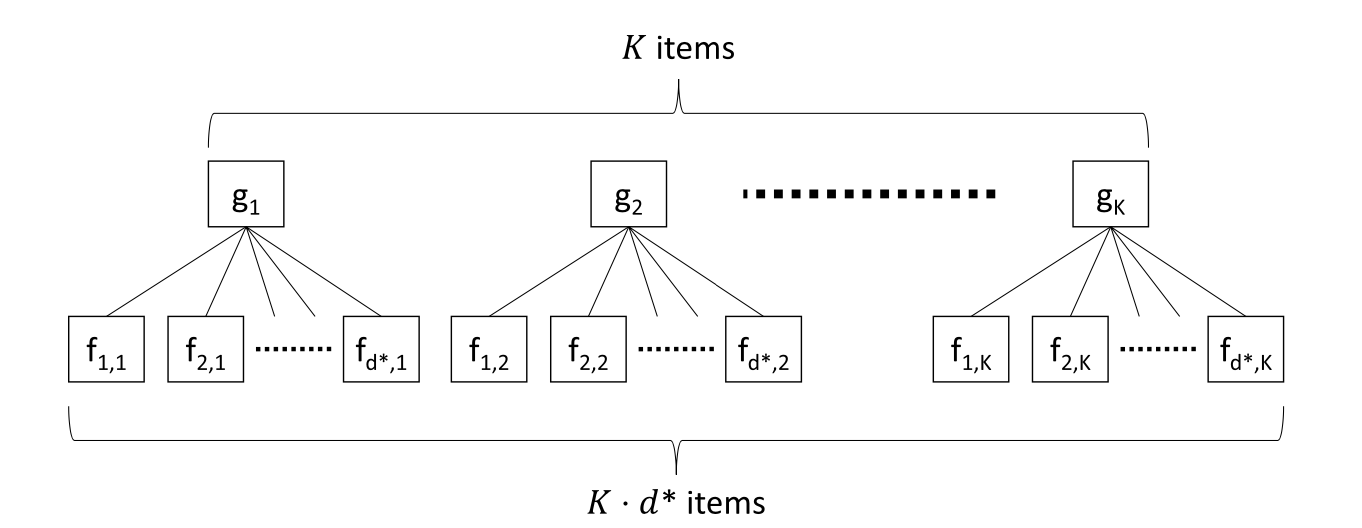
\includegraphics[width=0.75\textwidth]{Figures/DLNPR-Fig2}
	\caption{Illustration of the components of a function from $\calH^{(l)}$ [Lifted from the paper]}
	\label{fig:DLNPR-Fig2}
\end{figure}
Furthermore, let $N(\calH^{(l)})$ denote the number of linked two-layered networks from $\calF^{\text{(neural networks)}}_{M^*,d^*, d, \alpha}$ that define the functions from $\calH^{(l)}$. Then the following recursion holds: 
\begin{align*}
    N(\calH^{(0)}) &= 1,\\
    N(\calH^{(l)}) &= K + K\cdot d^* \cdot N(\calH^{(l-1)}),\hbox{ }\hbox{ }\hbox{ }\hbox{ }\hbox{ }l\in\SN
\end{align*}
which can be retraced following Figure \ref{fig:DLNPR-Fig2}. Above functions $g_1, \dots, g_K$ correspond to $K$ networks from $\calH^{(0)} =\calF^{\text{(neural networks)}}_{M^*,d^*, d, \alpha} $ and the $K\cdot d^*$ inner functions $f_{1,1},\dots, f_{d^*,K}$ originate from $\calH^{(l-1)}$, which leads to $K\cdot d^* \cdot N(\calH^{(l-1)})$ additional networks. 

Recursuve consideration yields
\begin{equation}
	\label{eq:DLNPR-7}
	N(\calH^{(l)}) = \sum_{t=1}^l {d^*}^{t-1}\cdot K^t + (d^*\cdot K)^l
\end{equation}
Consequently, a function from $\calH^{(l)}$ has at most 
\begin{equation}
	\label{eq:DLNPR-8}
	N(\calH^{(l)})\cdot W(\calF^{\text{(neural networks)}}_{M^*,d^*, d, \alpha})
\end{equation}
variable weights. Although this number of weights is exponential in the number of layers $l$, it can be controlled because a typical example of the technical systems which motivated Definition \ref{def:DLNPR-2} has only a moderate finite $l$. As explained in the definition, all typical assumptions for the regression function in the literature also correspond to a small $l$. 

Define $\tilde{m}_n$ as the least squares estimate 
\begin{equation}
	\label{eq:DLNPR-9}
	\tilde{m}_n(\cdot) = \arg \min_{h\in \calH^{(l)}} \frac{1}{n} \sum_{i=1}^n \left|Y_i - h(X_i)\right|^2
\end{equation}

For the result this needs to be truncated. Define the truncation operator $T_\beta$ with level $\beta > 0$ as 
\[T_\beta u = \begin{cases}
	u &\text{ if }|u|\leq \beta \\
	\beta \cdot \sign(u) &\text{ otherwise }
\end{cases}\]
Results requre a few additional properties on activation function, which are satisfied by many common activation functions (like the sigmoidal squasher) and they can be checked with arbitrary $N \in \SN_0$. Summarized in the next definition
\begin{definition}
	\label{def:DLNPR-3}
	A nondecresaing and Lipschitz continuous function $\sigma: \SR\rightarrow [0,1]$ is called \emph{$N$-admissable} if the following conditions hold
	\begin{enumerate}
		\item The function $\sigma$ is at least $N+1$ times differentiable with bounded derivatives. 
		\item A point $t_\sigma\in\SR$ exists where all derivatives up to the order $N$ of $\sigma$ are different from zero. 
		\item If $y > 0$, the relation $|\sigma(y) - 1| \leq \frac{1}{y}$ holds. If $y < 0$, the relation $|\sigma(y)| \leq \frac{1}{|y|}$ holds.
	\end{enumerate}
\end{definition}
\begin{theorem}[Main Result]
	\label{thm:DLNPR-1}
	Let $\{(X_i,Y_i)\}_{i=1}^n$ be independent and identically distributed random variables in $\SR^d\times\SR$ such that $\supp(X)$ is bounded and 
	\begin{equation}
		\label{eq:DLNPR-10}
		\mathbf{E}\exp(c_1 \cdot Y^2) < \infty, \footnote{This is basically saying that the moment generating function of $Y^2$ exists in some neighborhood around 0}
	\end{equation}
	for some constant $c_1 > 0$. Let $m$ be the corresponding regression function, which satisfies a $(p,C)$-smooth generalized hierarchical interaction model of order $d^*$ and finite level $l$ with $p = q+ s$ for some $q\in \SN_0$ and $s \in (0,1]$. Let $N\in \SN_0$ with $N\geq q$. Furthermore, assume that in Definition \ref{def:DLNPR-2}.b all partial derivatives of order less than or equal to $q$ of the functions $g_k, f_{j,k}$ are bounded. That is, assume that easch function $f$ satisfies
	\begin{equation}
		\label{eq:DLNPR-11}
		\max_{\substack{j_1,\dots,j_d \in \{0,1,\dots,q\}, \\ j_1+ \dots + j_d \leq q}} \left\Vert \frac{\partial^{j_1 + \dots + j_d}f}{\partial^{j_1}x^{(1)}\dots\partial^{j_d}x^{(d)}}\right\Vert \leq c_2
	\end{equation}
	and let all functions $g_k$ be Lipschitz continuous with Lipschitz constant $L> 0$ [which follows from (\ref{eq:DLNPR-11} if $q > 0$]. Let $\calH^{(l)}$ be defined as in (\ref{eq:DLNPR-6}) with $K, d, d^*$ as in the definition of $m$, $M^* = \left\lceil c_{56}\cdot n^{d^*}{2p + d^*}\right\rceil $. $\alpha = n^{c_{57}}$ for suffeciently large constants $c_{56}, c_{57} > 0$, and using an $N$-admissible $\sigma:\SR\rightarrow[0,1]$ according to Definition \ref{def:DLNPR-3}.Let $\tilde{m}_n$ be the least squares estimate defined by (\ref{eq:DLNPR-9}) and define $m_n = T_{c_3\log n}\tilde{m}_n$. Then 
	\[\mathbf{E}\int \left|m_n(x) - m(x)\right|^2 \mathbf{P}_X(dx) \leq c_4 \cdot \log^3(n) \cdot n^{-\frac{2p}{2p+d^*}}\]
	holds for suffeciently large $n$.
\end{theorem}
The authors include the following remarks on this main result
\begin{enumerate}
	\item For $p\geq 1$ and $C \geq 1$, the class of $(p,C)$-smooth generalized hierarchical interaction models of order $d^*$ satisfying the assumptions of the theorem contains all $(p,C)$-smooth functions, which depend on at most $d^*$ of its input components (because all functions in Def 2 can be chosen as projections). So, the rate of convergence in Theorem \ref{thm:DLNPR-1} is optimal up to some logarithmic factor, according to Stone (1982). 
	\item Some parameters of the estimate $m_n$, like $l, K$, or $d^*$ can be uknown in practice. They then would have to be chosen in a data dependent way. This has been studied in the literature apparently.
	\item Equation (\ref{eq:DLNPR-10}) in above theorem prevents heavy tails and ensure that the distribution of $Y$ is suffeciently concentrated in order to allow good estimates. 
\end{enumerate}
\begin{corollary}
	Suppose $\{(X_i,Y_i)\}_{i=1}^n$ is an i.i.d sample with values in $\SR^d\times\SR$ such that the support of $X$ is bounded and $\mathbf{E}\exp(c_1\cdot Y^2) < \infty$ for some constant $c_1 > 0$. Suppose the corresponding regression function $m$ satisfies a $(2,C)$-smooth generalized hierarchical interaction model of order 2 and finite level 0. Further assume that in Definition \ref{def:DLNPR-2}.b all partial derivatives of order $\leq 1$ of $g_k, f_{j,k}$ are bounded. Take $M^* = \left\lceil c_{56}n^{\frac{1}{3}}\right\rceil$. Use $\sigma(z) = \frac{1}{1+ \exp(-z)}$ and $\tilde m_n$ and $m_n$ as defined in Theorem \ref{thm:DLNPR-1}. Then
	\[\mathbf{E}\int \left|m_n(x) - m(x) \right|^2 \mathbf{P}_X(dx) \leq c_4\cdot\log^3(n)\cdot n^{-\frac{2}{3}},\footnote{Stringent conditions, but that is a wicked rate of convergence}\]
	holds for sufficiently large \(n\).
\end{corollary}
\begin{proof}
	Using notation from Theorem \ref{thm:DLNPR-1}, can choose $N = 1 = 1$. The sigmoidal squasher $\sigma$ is 1-admissible. Then the application of Theorem \ref{thm:DLNPR-1} implies the corollary.
\end{proof}

\subsection{Application to Simulated Data}

Section compares the neural net to an adaptive $k$-nearest neighbors appraoch as interpolation with radial basis function (\emph{RBF}). 
The paramaters $l, K, d^*, M^*$ of the neural network estimate (\emph{neural-x}) defined in Theorem \ref{thm:DLNPR-1}. To solve the least squares problem in (\ref{eq:DLNPR-9}). To solve the least squares problem use the quasi-Newton method of the function \emph{fminunc} in \emph{MATLAB} to approximate a solution.

Also compare this neural network estimate, which is characterized by the data-dependent choice of its structure and not completely connected neurons, to more ordinary fully connected neural networks with predefined numbers of layers but adaptively chosen numbers of neurons per layer.

Estimate outpreforms the other approaches in the three typical examples for generalized hierarchical interaction models. In these cases, the relative improvement of the estimate is larger with a larger sample size, which is an indicator of a better rate of convergence.

In some more extreme cases, this paper's approach is not always the best, though it still preforms will in some situations. In any case though, the results from simulation are promising. 

\subsection{Proofs}

Won't be covered in notes, but the proofs are given in section four of the paper and would be a good idea to examine.



\newpage
%!TEX root = /Users/manunavjeevan/Desktop/Research/ML + Lasso/Annotated Literature Review/litNotesML.tex

\section{NPR Using Deep Neural Networks \textit{\small Johannes Schmidt-Hieber (ArXiv, 2017)}}

Full paper title is ``Nonparametric regression using deep beural networks with ReLU activation function.'' Paper appeared on ArXiv in 2019 and (I believe) is due to appear in Annals at some point. It can be found \href{https://arxiv.org/pdf/1708.06633.pdf}{here}.

\subsection{Introduction}

In nonparametric regression model with random covariates in unit hypercube, observe $n$ i.i.d vectors $\mathbf{X}_i \in [0,1]^d$ and $n$ responses $Y_i \in \SR$ from the model $\vX$
\begin{equation}
	\label{eq:sh-1}
	Y_i = f_0(\mathbf{X}_i) + \eps_i
\end{equation}
The noise variables $\eps_i$ are assumed to be $i.i.d$ standard normal and independent of $\vX_i$. Statistical problem is to recover the unkown function $f_0: [0,1]^d\to\SR$ from the sample $(\vX, Y_i)_i$. Various methods exist that allow one to estimate the regression function nonparametrically, including kernel regression, smoothing, series estimators/wavelets, and splines. This paper considers fitting a multilayer feedforward artificial neural network to the data. Shown that estimator achieves nearly optimal convergence rates under various constraints on the regression function.

Deep neural networks have been used in practice from some time, but there is not much mathematrical understanding. Problem is that fitting a neural network to data is highly nonlinear in the parameters. Moreover, the function class is non-convex and various regularization methods are combined in practice. 

Article inspired by the idea to build a statistical theory that provides some understanding of these procedures. Method is too complex to be theoretically tractible, so some selection of important characteristics must be done in analysis. 

To fit a neural network, an activation function $\sigma: \SR\to\SR$ needs to be chosen. Traditionally, sigmoidal activation functions were employed (as in Secition \ref{sec:dl_npr}). For deep neural networks, however, there is a clear gain to using the non-sigmoidal rectifier linear unit (ReLU) 
\[\sigma(x) = \max(x,0) = (x)_+\]
In practice, ReLU outperforms other activation functions with regards to performance and computational cost. Statistical analysis for ReLU activation function is quite different from earlier approaches. Viewed as a nonparametric method, ReLU networks have some suprising properties. Deep networks with ReLU activation produce functions that are piecewise linear in the input. Nonparametric methods based on piecewise linear approacimations are typically not able to capture higher  order smoothness in the signal and are rate-optimal only up to smoothness index two. Paper shows that ReLU combined with deep network architecture achieves near minimax rates for arbitrary smoothness of the regression function. 

Number of hidden layers has been growing, results support this. Further, generally contain many more network parameters than sample size. Paper accounts for this by assuming number of potential nework parameters is much larger than the sample size. For noisy data generated from the nonparameteric regression model, overfitting leads to generalization errors and incorporating regularization becomes esential.

Existing statistical theoery often requires that the size of the network parameteres tends to infinity as the sample size increases. In practice, estimated network weights are, however, rather samll. Paper incorporates this into theory, procing it is suffecient to consider neural networks with all network parameters bounded in absolute value by one. 

Still, NPR using deep neural nets has to get around the curse of dimensionality. Paper gets around this by imposing the generalized hierarchical model structure. 

\subsection{Mathematical Definition of Multilayer Neural Networks} 

\paragraph{Neural Network}

Fitting a nerual network requires the choice of an activatino function $\sigma: \SR\to\SR$ and the network architecture. Paper studies the ReLU activation funtion 
\[\sigma(x) = \max(x,0)\]
For $\mathbf{v} = (v_1, \dots, v_r)$ define the shifted activation function $\sigma_{\mathbf{v}}: \SR^r\to\SR^r$ as 
\[\sigma_{\mathbf{v}}\begin{pmatrix}y_1 \\ \vdots \\y_r\end{pmatrix} = \begin{pmatrix} \sigma(y_1 - v_1 )\\    \vdots \\ \sigma(y_r - v_r) \end{pmatrix}\]
The network architecture $(L, \vp)$ consists of a positive integer $L$ called the number of hidden layers or \emph{depth} and a \emph{width vector} $\vp \in \SN^{L+2}$. So a neural network with network architecture $(L, \vp)$ is then any function of the form 
\begin{equation}
	\label{eq:sh-2}
	f:\SR^{p_0}\to\SR^{P_{L+1}}, \hbox{ }\hbox{ }\hbox{ }\vx\mapsto f(\vx) = W_l \sigma_{\vv_L} W_{L-1}\sigma_{\vv_{l-1}}\cdots W_1\sigma_{\vv_1}W_0\vx
\end{equation}
where $W_i$ is a $p_i \times p_{i+1}$ weight matrix and $\vv_i \in \SR^{p_i}$ is a shift vector. Network functions are therefore built by alternating matrix-vector multiplications with the action of the non-linear activation functions $\sigma$. In (\ref{eq:sh-2}) it is also possible to omit the shift vectors by considering the input $(\vx, 1)$ and enlarging the weight matrices by one row and one column with appropriate entries. 

In the compsci literature, neural networks are more commonly introduced via their representation as directed acyclic graphs, like in a figure above in section \ref{sec:dl_npr}.

\paragraph{Mathematical Modeling of Deep Network Characteristics} 

Given a network function \(f(\vx)\) as defined in (\ref{eq:sh-2}), the network parameters are the entries of the matricies $(W_j)_{j = 0,\dots, L}$ and the vectors $(\vv_j)_{j = 0,\dots, L}$. These parameters need to be estimated/learned from the data. 

Aim of this article is to consider a framework that incorporates essential features of modern deep network architectures. Allow for large depth $L$ and large number of potential network parameter. Thus, consider high dimensional settings with more parameters that training data. 

Another characteristic of trained networks is that the size of the learned network parameters is typically not very large. Common network initialize the weight matrices $W_j$ by a nearly orthogonal random matrix if two succesive layers have the same width. IN practice, the trained network weights are typically not far from the initialized weights. In an orthogonal matrix, all entries are bounded in absolute value by one, this explains that also the trained network weights are not large. 

Existing theory requires that the size of the network parameters tends to infinity. If large parameters are allowed, one can easily approximate step functions by ReLU networks. To be more in line with what is observed in practice, consider networks with all parameters bounded by one. Constraint can easily be build into the deep learning algorithm by projecting the network parameters in each iteration onto the interval [-1,1].

If $\|W_i\|_{\infty}$ denotes the sup-norm of $W_j$, the space of network functions with given network architecture and network parameters bounded by one is 
\begin{equation}
	\label{eq:sh-3}
	\calF(L,\vp) := \left\{ f\text{ of the form (\ref{eq:sh-2}) }: \max_{j= 0,\dots, L} \|W_j\|_\infty \vee |\vv_k|_\infty \leq 1 \right\}
\end{equation}
with the coefficeint that $\vv_0$ is a vector of coefficients all equal to zero. 

In deep learning, sparsity of the neural network is enforced through regularization or specific forms of networks. Dropout, for instance, randomly sets units to 0 and has the effect that each unit will be active only for a small fraction of the data. In the notation of this paper, this means that each of the vectors $\sigma_{\vv_k}W_{k=1}\cdots W_1\sigma_{\vv_1}W_0\vx$, $k= 1,\dots, L$ is zero over a large range of the input space $x\in [0,1]^d$.  Convolutional neural networks filter the input over local neighborhoods. Rewritten in the form (\ref{eq:sh-2}), this essentially means that the $W_i$ are banded Toeplitz matrices\footnote{A Toeplitz matrix is one where each descending diagonal from left to right is constant. For example \[\begin{pmatrix}a & b & c \\ d & a & b \\ e & d & a\end{pmatrix}\] is a Toeplitz matrix. An $l$ banded Toeplitz matrix is one such that only the middle $l$ diagonals of the matrix are non-zero. For example, a traditional diagonal matrix is a $1$ banded Toeplitz matrix}. All network parameters corresponding to higher off-diagonal entries are thus set to zero. 

This paper models sparsity by asusming that there are only a few non-zero / active network parameters. If \(\|W_j\|_0\) denotes the number of non-zero entries, then the $s$-sparse networks are given by 
\begin{equation}
\begin{split}
	\label{eq:sh-4}
	\calF(L, \vp, s) &:= \calF(L, \vp ,s, F) \\
	&:= \left\{f\in \calF(L, \vp): \sum_{j=0}^L \|W_j\|_0 + |\vv_j|_0 \leq s, \|f\|_\infty \leq F \right\}
\end{split}
\end{equation}
The upper bound on the uniform/sup norm of $f$ is most of the time not needed and omitted in the notation. Consider cases where the number of network parameters $s$ is small compared to the total number of parameters in the network. 

To estimate the parameters of the model, it is common to apply variations of stochastic gradient descent combined with other techniques such as dropout to the loss induced  by the log-likelihood. For nonparametric regression with normal errors, this coincides with the least-squares loss. The common objective of all reconstruction methods is to find networds $f$ with a small empirical risk $\frac{1}{n}\sum_{i=1}^n (Y_i - f(\vX_i))^2$. For any estimator $\hat{f}_n$ that returns a network in the class $\calF(L,\vp, s, F)$ define the correspoinding quantity 
\begin{equation}
	\label{eq:sh-5}
	\Delta_n(\hat{f}_n, f_0) := \E_{f_0}\left[\frac{1}{n}\sum_{i=1}^n (Y_i - \hat{f}_n(\vX)_i)^2 - \inf_{f\in\calF(L,\vp, s, F)} \frac{1}{n} \sum_{i=1}^n (Y_i - f(\vX)_i)^2\right]
\end{equation}
The sequence $\Delta_n(\hat{f}_n , f_0)$ measures the difference between the expected empirical risk of $\hat{f}_n$ and the global minimum over all networks in the class. The subscript $f_0$ indicates that the expectation is taken with respect to the sample generated from the nonparametric regression model with regression function $f_0$. In general $\Delta_n (\hat{f}_n, g_0) \geq 0$ and $\Delta_n(\hat{f}_n, f_0) = 0$ if $\hat{f}_n$ is an empirical risk minimizer. Note here this is just measuring the ``distance'' between the estimation technique and the global minimumum. 

To evaluate the statistical performance of an estimator $\hat{f}_n$, derive bounds for the prediction error 
\[R(\hat{f}_n, f_0) := \E_{f_0}\left[\left(\hat{f}_n(\vX)-f_0(\vX)\right)^2\right]\]
The term $\Delta_n(\hat{f}_n, f_0)$ can be related via empirical process theory to a constant times $(R(\hat{f}_n, f_0)-R(\hat{f}_n^{\text{ERM}}, f_0))$ plus a remainder, where $\hat{f}_n^{\text{ERM}}$ being an empirical risk minimizer. So $\Delta_n(\hat{f}_n, f_0)$ in $n$ for commonly employed methods such as stochastic gradient descent is an interesting problem in its own. Only skech a possible proof strategy here: 
\begin{enumerate}
	\item Because of potentially local minima and saddle poins, gradient descent bethods only have a small chance to reach the global minimum w/o getting stuck in a local minimum first
	\item Making a link to sperical spin glasses, paper cited provides a heuristic suggesting that the loss of any local minima lies in a band that is lower bounded by the loss of the global minimum
	\item Width of the band depends on the width of the network, if the heuristic argument can be made rigorous then the width of the band provides an upper bound for $\Delta_n(\hat{f}_n, f_0)$ for all methods that converge to a local minumum 
\end{enumerate}
This would allow study of deep learning without an explicit analysis of the algorithm. 

\subsection{Main Results}

Theoretical performance of neural networks dpends on the underlying function class. Classical appraoch in nonparametric statistics is to assume that the regression function is $\beta$-smooth. The minimax estimation rate for the prediction error is then 
\[n^{-2\beta/(2\beta + d)}\]
Since the input dimension $d$ in neural network applications is very large, these rates are extremely slow. The huge sample sizes often encountered in these applications are by far not sufficient to compensate the slow rates.  With this in mind, consider a function class that is natural for neural nrwtorks and exhibits some low-dimensional structure that leads to input dimension free exponents in the esimation rates. 

Assume that the regression function $f_0$ is a composition of several functions, that is, 
\begin{equation}
	\label{eq:sh-6}
	f_0 = g_q\circ g_{q-1} \circ \dots \circ g_1 \circ g_0
\end{equation}
with $g_i:[a_i,b_i]^{d_i} \to [a_{i+1}, b_{i+1}]^{d_{i+1}}$. Denote by $g_i = (g_{ij})^T_{j=1,\dots,d_{i+1}}$the components of $g_i$ and let $t_i$ be the maximal number of variables on which each of the $g_{ij}$ depends on. Thus, without loss of generality, each $g_{ij}$ is a $t_i$ variate function. As an example, consider the function $f_0(x_1, x_2, x_3) = g_{11}(g_{01}(x_3), g_{02}(x_2))$ for which $d_0 = 3$, $t_0= 1$, $d_1 = t_1 = 2$, and $d_2=1$. 

Always must have $t_i \leq d_i$, and for certain constraints, such as in additive models, $t_i$ mught be much smaller than $d_i$.  The single components $g_0, \dots, f_1$ and the pairs $(\beta_i, t_i)$ are clearly not identifiable. As we are only interested in estimation of $f_0$, this causes no problems. Among all possible representations, one should pick the one that leads to the fastest estimation rate. 

In the $d$-variate regression model (\ref{eq:sh-1}), $f_0: [0,1]^d\to\SR$ and thus $d_0 = d$, $a_0 = 0$, $b_0 = 1$, and $d_{q+1} = 1$. One should keep in mind that (\ref{eq:sh-6}) is an assumption on the regression function that can be made independently of whether neural networks are used to fit the data or not. In particular, the number of layers $L$ in the network need not be the same as $q$. 

Conceivable that for many of the problems for which neural networks perform well, a hidden hierarchical input-output relationship of the form (\ref{eq:sh-6}) is present with small values $t_i$. Slightly more specific function spaces, which alternate between summations and compositions of functions have been considered (the paper in Section \ref{sec:dl_npr}) is an example of one of these). 

A function has Hölder smoothness index $\beta$ if all partial derivatives up to order $\lfloor \beta \rfloor$ exist and are bounded, and the partial derivatives of order $\lfloor \beta \rfloor$ are $\beta - \lfloor \beta \rfloor$ Hölder. The ball of $\beta$-Hölder functions with raduis $K$ is then defined as 
\[\calC_r^\beta(D,K) = \left\{f:D\subset\SR^r\to\SR: \sum_{\valpha : |\valpha| < \beta|} \|\partial^\valpha f\|_\infty + \sum_{{\valpha}: |\valpha|= \lfloor\beta\rfloor} \sup_{\substack{\vx,\vy \in D \\ \vx \neq \vy}}\right\}\]

Assume that each of the functions $g_{ij}$ has Hölder smoothness $\beta_i$. Since $g_{ij}$ is also $t_i$-variate, $g_{ij}\in \calC_{t_i}^{\beta_i}\left([a_i,b_i]^{t_i}, K_i\right)$ and the underlying function space becomes
\begin{align*}
	\calG(q,\vd,\vt,\bm{\beta}, K) := \bigg\{f = g_q \circ \dots \circ g_0: g_i = (g_{ij})_j: [a_i,b_i]^{d_i}\to [a_{i+1}, b_{i+1}]^{d_{i+1}}&, \\g_{ij}\in \calC_{t_i}^{\beta_i}\left([a_i,b_i]^{t_i}, LK\right), \text{ for some }|a_i|, |b_i| \leq K&\bigg\}
\end{align*}
with $\vd := (d_0, \dots, d_{q+1})$, $\vt:=(t_0, \dots, t_q)$, $\bm{\beta}:= (\beta_0, \dots, \beta_q)$. 

For estimation rates in the nonparametric regression model, the crucial quantity is the smoothness of $f$. Imposing smoothness on the functions $g_i$, one must be find the induced smoothness of $f$, for comparasion on the minimax rates, etc. If, for instance, \(q =1, \beta_0, \beta_1\leq 1\), and \(d_0 = d_1 = t_0 =t_1 = 1\) and $f$ has smoothness $\beta_0, \beta_1$, then one should be able to achieve at lest the convergence rate 
\(n^{-2\beta_0\beta_1/(2\beta_0\beta_1 + 1)}\)

For $\beta_1 > 1$, this rate changes. Below will show that the convergence of the network estimator is described by the effective smoothness indices 
\[\beta_i^* := \beta_i \prod_{\ell = i+1}^q (\beta_{\ell} \wedge 1 )\]
via the rate 
\begin{equation}
	\label{eq:sh-7}
	\phi_i := \max_{i = 0,\dots, q} n^{-\frac{2\beta_i^*}{2\beta_i^* + t_i}}
\end{equation}
Recalling the definition of $\Delta_n(\hat{f}_n, f_0)$ in (\ref{eq:sh-5}). 

\begin{theorem}[Main Result]
	\label{thm:sh-1}
	Consider the d-variate nonparametric model in (\ref{eq:sh-1}) for composite regression function (\ref{eq:sh-6}) in the class $\calG(q, \vd, \vt, \bm{\beta}, K)$. Let $\hat{f}_n$ be an estimator taking values in the network class $\calF(L, (p_i)_{i=0, \dots, L+1}, s, F)$ satisfying 
	\begin{enumerate}
		\item $F\geq \max(K,1)$
		\item $\sum_{i=0}^q \log_2(4t_i \vee 4\beta_i)\log_2 n\leq L \lesssim n \phi_n$\footnote{From what I understand, the notation $\lesssim f_n$ means $o(f_n)$ whereas the notation $\asymp f_n$ means $O(f_n)$}
		\item $n\phi_n \lesssim \min_{i=1,\dots,L}p_i$
		\item $s\asymp n\phi_n \log n$
	\end{enumerate}
	Then there exist constants $C, C'$ only depending on $q, \vd, \vt, \bm{\beta}, F$ such that if $\Delta_n(\hat{f}_m, f_0)\leq C\phi_n L \log^2(n)$ then 
	\begin{equation}
		\label{eq:sh-8}
		R(\hat{f}_n, f_0)\leq C'\phi_nL\log^2 n 
	\end{equation}
	and if $\Delta_n(\hat{f}_n,f_0)\geq C\phi_n L \log^2 n$ then 
	\begin{equation}
		\label{eq:sh-9}
		\frac{1}{C'}\Delta_n (\hat{f}_n, f_0) \leq R(\hat{f}_n, f_0) \leq C'\Delta_n(\hat{f}_n, f_0)
	\end{equation}
\end{theorem}

In order to minimize the rate $\phi_n L \log^2 n$ the best choice is to choose $L$ of the order $\log_2 n$. The rate in the regime $\Delta_n (\hat{f}_n, f_0)\leq C'\phi_n\log^3n$ becomes then 
\[R(\hat{f}_n,f_0)\leq C'\phi_n \log^3 n\]
Convergence rate in Theorem \ref{thm:sh-1} depends on $\phi_n$. Below will show that $\phi_n$ is a lower bound for the minimax estimation risk over this class. The term $\Delta_n(\hat{f}_m,f_0)$ is large if $\hat{f}_n$ has a large empirical risk compared to the empirical risk minimizer. Having this term in the convergence rate is unavoidable as it also wppears in the lower bound derived in (\ref{eq:sh-9}). Since for the empirical risk minimizer the $\delta_n$-term is zero by definition, we have the following direct consequence of the main theorem. 
\begin{corollary}
	\label{cor:sh-1}
	Let $\tilde{f}_n \in \argmin_{f\in\calF(L,\vp,s,F)} \sum_{i=1}^n(Y_i - f(\vX_i))^2$ be the empirical risk minimizer. Under the same conditions as for Theorem \ref{thm:sh-1}, there exists a constant $C'$ only depending on $q,\vd,\vt,\vbeta$ such that 
	\begin{equation}
		\label{eq:sh-10}
		R(\tilde{f}_n,f_0) \leq C'\phi_n L \log^2 n
	\end{equation}
\end{corollary}
Condition (i) in Theorem \ref{thm:sh-1} is mild and only states that the newtwork functions should have at least the same supremum norm as the regression function. From the other assumptions in Theoream \ref{thm:sh-1} it becomes clear that there is a lot of flexibility in picking a good network architecture as long as the number of active parameters is of the ``right'' order. To choose a network depth $L$ is is suffecient to have an upper bound on the $t_i \leq d_i$ and the smoothness indices $\beta_i$. Network width can be chosen independent of the smoothness indices by taking, for instance $n\lesssim \min_i p_i$.

Maybe possible to choose the sparsity $s$ adaptibely. From a practical point of view it is concievable but left to future work. 

Number of network parameters in a fully connected network is of the order $\sum_{i=0}^L p_i p_{i+1}$. This shows that Theorem \ref{thm:sh-1} requires sparse networks (since it requires a condition on $L$). For clearness of exposition, Theorem \ref{thm:sh-1} is stated without explicit constants, the proofs, however, an non-asymptotic. It is well-known that depe learning outperforms other methods only for long sample size. This indicated that the method may be able to adapt to underlying structure in the signal and thereform achieving fast convergence rates but with large constants or remainder terms which spoil the results for small samples. 

Proof of the risk bounds in Theorem \ref{thm:sh-1} is based on the following oracle-type inequality
\begin{theorem}
	\label{thm:sh-2}
	Consider the $d$-variate nonparametric regression model specified in (\ref{eq:sh-1}) with unkown regression function $f_0$ satisfying $\|f_0\|_\infty \leq F$ for some $F\geq 1$. Let $\hat{f}_n$ be any estimator taking values in the class $\calF(L,\vp,s,F)$ and let $\Delta_n(\hat{f}_n,f_0)$ be the quantity defined in (\ref{eq:sh-5}). For any $\eps\in(0,1]$ there exists a constant $C_\eps$ depending only on $\eps$ such that with 
	\[\tau_{\eps,n} := C_\eps F^2 \frac{(s+1)\log\left(n(s+1)^Lp_0p_{L+1}\right)}{n}\]
	we have 
	\begin{dmath*}
		(1-\eps)^2\Delta_n(\hat{f}_n,f_0) -\tau_{\eps,n} \leq R(\hat{f}_n,f_0) \leq (1+\eps)^2 \left(\inf_{f\in\calF(L,\vp,s,F)} \|f-f_0\|^2_{\infty} + \Delta_n(\hat{f}_n,f_0)\right) +\tau_{\eps,n}
	\end{dmath*}
\end{theorem}
A consequence of the oracle inequality is that the upper bounds on the risk become worse as the number of later increases. This is consistent with what has been observed in practice. 

An inspection of the proof shows two specific properties of the ReLU function is used. One of the advantages of deep ReLU networks is the projection property 
\begin{equation}
	\label{eq:sh-11}
	\sigma \circ \sigma = \sigma
\end{equation}
that can be used to pass a signal without change through several layers in the network. This is important since the approximation theory is based on the construction of smaller networks for simpler tasks that may not all have the same network depth. To combine these subnetworks into one needs to synchronzie network depths by adding hidden layers that do not change the output.

Another advantage of the ReLU activation is that all network parameters can be taken to be bounded in absolute value by one. If all network parameters are initialized by a value in [-1,1], this means that each network parameters only need to be varied by at most two during training. It is unclear whether results in the literature for non ReLU acrivation functions hold for bounded network parameters. 

The $L\log^2 n $ factor in the convergence rate $\phi_n L\log^2 n$ is likely an artifact of the proof. Nexgt show that $\phi_n$ is a lower bound for the minimax estimation risk over the class $\calG(q,\vd, \vt,\vbeta, K)$ in the interesting case that $t_i \leq \min (d_0, \dots, d_{i-1})$ for all $i$. This means that no dimensions are added on deeper abstraction levls in the composition of functions. 

\begin{theorem}
	\label{thm:sh-3}
	Consider the nonparameteric regression model (\ref{eq:sh-1}) with $\vX_i$ drawn from a distribution with Lebesgue density on $[0,1]^d$ which is lower and upper bounded by positive constants. For any non-negative integer $q$, any dimension vectors $\vd$ and $\vt$ satisfying $t_i\leq \min(d_0, \dots, d_{i=1})$, any smoothness vector $\vbeta$ and all sufficiently large constants $K>0$, there exists a positive constant $c$ such that 
	\[\inf_{\hat{f}_n} \sup_{f_0\in \calG(q,\vd,\vt,\vbeta,K)} R(\hat{f}_n, f_0) \geq c \phi_n\]
	where the $\inf$ is taken over all estimators $\hat{f}_n$\footnote{This shows that $\phi_n$ is a lower bound on minimax rate of convergence for estimators}
\end{theorem}
Proof is in appendix. Main ideas are sketched
\begin{enumerate}
	\item For simplicity, assume that $t_i = d_i = 1$ for all $i$. In this case, the functions $g_i$ are all univariate and real-valued. Define $i^* \in \arg\min_{i=0,\dots,q} \beta^*_i/(2\beta^*_i + 1)$ as an index for which estimation rate is obtained. 
	\item For any $\alpha > 0, x^\alpha$ has Hölder smoothness $\alpha$ and for $\alpha = 1$ the function is infintely differentiable and has finite Hölder norm for all smoothness indices.\footnote{Holder norm with smoothness index $\beta$ over a class of functions defined over $\Omega$ and into $\SR$, $$ \|f\|_{1,\beta} = \sup_{x\in\Omega} |f(x)| + \sup_{x\in\Omega} |f'(x)| + \sup_{\substack{x,y\in\Omega \\ x\neq y}} \frac{|f'(x) - f'(y)|}{\|x-y\|^\beta}$$}.Set $g_\ell (x) = x$ for $\ell < i^*$ and $g_\ell(x)$ = $x^{\beta_\ell \wedge 1}$ for $\ell > i^*$. Then 
	\[f_0(x) = g_1 \circ g_{q-1} \circ \dots \circ g_1 \circ g_0(x) = \left(g_{i^*}(x)\right)^{\prod_{\ell = i^* + 1}^q \beta_\ell \wedge 1}\]
	\item Assuming a uniform random design (errors distributed the same), the Kullback-Leibler divergence is $KL(P_f, P_g) = \frac{n}{2}\|g-f\|^2_2.$\footnote{Kullback-Leibler divergence is a measure of how ``far apart'' probability distributions are. If $P$ and $Q$ are probability distributions over a set $\calX$, and $P$ is absolutely continuous with respect to $Q$, then the Kullback-Leibler divergence from $Q$ to $P$ is defined as 
	\[KL(P_f, P_g) = \int_\calX \log\left(\frac{dP}{dQ}\right)dP\] where $\frac{dP}{dQ}$ is the density (Radon-Nikodym derivative) of $P$ with respect to $Q$.} Take a kernel function $K$ and consider $\tilde{g}(x) = h^{\beta_{i^*}} K (x/h)$. Under standard assumptions on $K$, $\tilde{g}$ has Hölder smoothness index $\beta_{i^*}$.
	\item  Now can generate two hypotheses $f_{00}(x)=0$ and $f_{01}(x) = (h^{\beta_{i^*}}K(x/h))^{\prod_{\ell = i^* + 1}^q \beta_\ell \wedge 1}$ by taking $g_{i^*}(x) = 0$ and $g_{i^*}(x) = \tilde{g}(x)$. Therefore, because our domain bounds $x \in [0,1]$: $\vert f_{00}(0) - f_{01}(0)\vert\hbox{}\gtrsim h^{\beta_{i^*}}$ assuming that $K(0) > 0$. 
	\item For the Kullback-Leibler divergence, find $KL(P_{f_{00}}, P_{f_{01}}) \lesssim nh^{2\beta_{i^*}^* + 1}$. Using a theorem 2.2 from the book \textit{Introduction to nonparametric estimation} (Tsybakov 2009), this shows that the poitwise rate of convergence is 
	\[n^{-2\beta_{i^*}^*/(2\beta_{i^*}^* + 1)} = \max_{1 = 0,\dots, q} n^{-2\beta_i^*/(2\beta_i^* +1)}\]
	which matches with the upper bound since $t_i = 1$ for all $i$. For lower bound on the prediction error, generalize argument to a multiple testing problem.
\end{enumerate}
$L^2$-minimax rate coincides in most regimes with the sup-norm rate obtained for composition of two functions. But unlike the classical nonparameteric regression model, the minimax estimation rates for $L^2$-loss and sup-norm loss differ fot some setups by a polynomial power. There are several results in approximation theory that provide lower bounds on the number of required network weights $s$ such that all functions in a function class can be approximated by a $s$-sparse network up to some prescribed error. Results of this flavor can also be quite easily derived by combining the minimax lower bound with the oracle inequality. Argument is that if the same approximaation rates would hold for networks with fewer parameters, we would obtain rates that are faster than the minimax rates.
\begin{lemma}
	\label{lemma:sh-1}
	Given $\beta, K > 0, d\in\SN$, there exists constants $c_1, c_2$ only depending on $\beta, K, d$ such that if 
	\[s\leq c_1 \frac{\eps^{-d/\beta}}{L\log(1/\eps)}\]
	for some $\eps \leq c_2$, then for any width vector $\vp$ with $p_0 = d$ and $p_{L+1} = 1$
	\[\sup_{f_0\in \calC_d^\beta([0,1]^d, K)} \inf_{f\in\calF(L,\vp,s)} \geq \eps\]
\end{lemma}
This, I guess, helps establish some lower bound. 


\newpage
%!TEX root = /Users/manunavjeevan/Desktop/Research/ML + Lasso/Annotated Literature Review/litNotesML.tex

\section{Central Limit Theorems and Bootstrap in High Dimensions \textit{\small Victor Chernozhukov, Denis Chetverikov, Kengo Kato (A0P 2017)}}

Article appeared in Annals of Probability in 2017. It can be found through the AoP website \href{https://projecteuclid.org/euclid.aop/1502438428}{here} or from ArXiv \href{https://arxiv.org/pdf/1412.3661.pdf}{here}.

Paper derives central limit theorems and bootstrap theorems for probabilities that sums of centered high dimensional random vectors hit hyperrectangles and sparsely convex sets. 

\subsection{Introduction}

Let $X_1, \dots, X_n$ be independent random vectors in $\SR^p$ where $p\geq 3$ may be large or even much larger than $n$. Denote by $X_{ij}$ the $j$-th coordinate of $X_i$ so that $X_i = (X_{i1},\dots,X_{ip})'$. Assume that each $X_i$ is centered, so that $\E[X_ij] = 0$ and $\E[X_{ij}^2] < \infty$ for all $i = 1, \dots, n$ and $j = 1, \dots, p$. Define the normalized sum 
\[S_n^X := \left(S_{n1}^X, \dots, S_{np}^X\right)' := \frac{1}{\sqrt{n}} \sum_{i=1}^n X_i\]
Paper considers Gaussian approximations to $S_n^X$ and, to this end, let $Y_1, \dots, Y_n$ be independent centered Gaussian random vectors in $\SR^p$ such that each $Y_i$ has the same covariance matrix as $X_i$, that is $Y_i \sim N(0,\E[X_iX_i'])$. Define the normalized sum for the Gaussian random vectors 
\[S_n^Y := \left(S_{n1}^Y, \dots, S_{np}^Y\right)' := \frac{1}{\sqrt{n}}\sum_{i=1}^n Y_i\]
Interested in bounding the quantity 
\begin{equation}
	\label{eq:cck17-1}
	\rho_n(\calA) := \sup_{A\in \calA}\left| \P(S_n^X \in A) - \P(S_n^Y\in A)\right|
\end{equation}
where $\calA$ is a class of Borel sets in $\SR^p$. Section 2 derives this bound for $\calA = \calA^{\text{re}}$, the class of all byperrectangles ans shows that this bound vconverges to 0 under some conditions. 

Bounding $\rho_n(\calA)$ for various classes $\calA$ of sets in $\SR^p$ with a special emphasis on explicit dependence on the dimension $p$ in the bounds has been studied. The appendix for the 2013 Annals of Statistics Paper, ``Gaussian approximations and multiplier bootstrap for maxima of sums of high dimensional random vectors'' also by Chernozhukov, Chetverkiov, Kato offers a literature review. 

\paragraph{Some Notation} 

Use notation $\|v\|_0 = \sum_{j=1}^p \mathds{1}\{v_j\neq 0\}$ and $\|v\| = (\sum_{j=1}^p v_j^2)^{1/2}$. For $\alpha > 0$, defined the function $\psi_a :[0, \infty) \to [0, \infty)$ by $\phi_\alpha := \exp(x^\alpha) - 1$. Consider 
\[ \|\xi\|_{\psi_\alpha} := \inf \{\lambda > 0: \E[\psi_\alpha(|\xi|/\lambda)] \leq 1 \} \]
For $\alpha \in [1,\infty)$ this is a well defined norm, whereas for $\alpha \in (0,1)$ this is a quasi-norm. That is, there exists a constant $K_\alpha$ depending only on $\alpha$ such that 
\[\|\xi_1 + \xi_2\|_{\psi_\alpha} \leq K_\alpha (\|\xi_1\|_{\psi_\alpha} + \|\xi_2\|_{\psi_\alpha})\]
Throughout the paper assume $n\geq 4$ and $p \geq 3$

\subsection{High-dimensional CLT for hyperrectangles}

Begin by presenting an abstract theorem. General but depends on the tail properties of the distributions of the coordinates of $X_i$ in a nontrivial way. Next, apply this theorem under simple moment conditions and derive more explicit bounds. 

Let $\calA^{\text{re}}$ be the class of all hyperrectangels in $\SR^p$; that is $\calA^{\text{re}}$ consists of all sets $A$ of the form 
\begin{equation}
	\label{eq:cck17-4}
	A = \{w \in \SR^P: a_j \leq w_j \leq b_j\text{ for all }j = 1, \dots, p\}
\end{equation}
for some $-\infty \leq a_j \leq b_j \leq \infty$, $j = 1, \dots, p$. Will derive a bound on $\rho_n(\calA^{\text{re}})$ and show that, under certain conditions it converges to 0, even in the high dimensional setting. 

To describe the bound, need to prepare some notation. Define 
\[L_n := \max_{1\leq j \leq p} \sum_{i=1}^n \E\left[|X_{ij}|^3\right]/n\]
and for $\phi \geq 1$, define for $Z = X,Y$
\begin{equation}
	\label{eq:cck17-5}
	M_{n,Z}(\phi) := n^{-1}\sum_{i=1}^n \E\left[\max_{1\leq j \leq p}\mathds{1}\left\{\max_{1\leq j \leq p} |X_{ij}| < \sqrt{n}/(4\phi\log p)\right\}\right]
\end{equation}
and let 
\[M_n(\phi) := M_{n,X}(\phi) + M_{n,Y}(\phi)\]
The following is the main result of the paper 
\begin{theorem}[Abstract high-dimensional CLT for hyperrectangles]
	\label{thm:ckk17-1}
	Suppose that there exists some constant $b > 0$ such that $n^{-1}\sum_{i=1}^n \E[X_{ij}^2] \geq b$ for all $j = 1, \dots, p$. Then tere exist constants $K_1, K_2 > 0$ depending only on $b$ such that, for every constant $\bar{L}_n \geq L_n$,
	\begin{equation}
		\label{eq:cck17-6}
		\rho_n(\calA^{\text{re}}) \leq K_1 \left[\left(\frac{\bar{L}^2_n\log^7 p}{n}\right)^{\frac{1}{6}} + \frac{M_n(\phi_n)}{\bar{L}_n}\_\right]
	\end{equation}
	with 
	\begin{equation}
		\label{eq:cck17-7}
		\phi_n := K_2\left(\frac{\bar{L}_n^2 \log^4 p}{n} \right)^{-\frac{1}{6}}
	\end{equation}
\end{theorem}


\newpage
%!TEX root = /Users/manunavjeevan/Documents/GitHub//mnavjeev.github.io/files/ML + Lasso/Annotated Literature Review/litNotesML.tex

\section{Sparse Principal Component Analysis \textit{\small Hui Zou, Trevor Hastie, Robert Tisbirani (JCGS, 2006)}}

Paper appeared in Journal of Computational and Graphical Statistics in 2006. Extends PCA to the high dimensional setting so there is consistency when $p \gg n$. 

\subsection{Introduction}

Principal Component Analysis is a popular data-processing and dimension reduction technique, with many applications in engineering, biology, and social science. PCA seeks the linear combinations of the original variables such that the derived variables capture maximal variance. It can be computed via the singular value decomposition (SVD) of the data matrix. 

In detail, let the data $\vX$ be an $n\times p$ matrix, where $n$ and $p$ are the number of observations and the number of variables, respectively. Without loss of generality, assume the column means of $\vX$ are all zero and let the SVD of $\vX$ be 
\begin{equation}
	\label{eq:scpa-1.1}
	\vX = \vU \vD \vV^T
\end{equation}
where $\vZ = \vU\vD$ are the principle components and the columns $\vV$ are the corresponding loadings of the principal components. The sample variance of the $i^{th}$ PC is $\vD^2_{ii}/n$. In gene expression data the standardized PCs $\vU$ are called the \emph{eigen-arrays} and $\vV$ are called the \emph{eigen-genes}. Usually the first $q$, $q \ll \min(n,p)$, principal components are used to represent that data, and so a dimensionality reduction is achieved. 

Success of PCA is due to the following important properties: 
\begin{enumerate}
 	\item Principal components sequentially capture the maximum variability among the columns of $X$, guarenteeing minimal information loss.
 	\item Principal components are uncorrelated, so we can talk about one principal component without referring to others
 \end{enumerate} 

However, PCA also has an obvious drawback, that is, each PC is a linear combination of $p$ variables and the loadings are typically non-zero. This makes it difficult to interpret the derived PCs. Rotation techniques are commonly used to help practitioners interpret the derived PCs, Joliffe (1995). Vines (2000) considered simple principal components by restricting the loadings to take values from a small set of allowable integers such as $0, 1$, and $-1$.

Feel it is desirable not only to achieve the dimensionality reduction, but also reduce the number of explicitly used variables. Ad-hoc way to achieve this is to artificially set the loadings with absolute values smaller than a threshold to zero. The same interpretation issues arise in multiple linear regression, where the response is predicted by a linear combination of the predictors in lasso. 

This article introduces a new approach for estimating PCs with sparse loading, which we call sparse principal component analysis. SPCA is built on the fact that a PCA can be written as a regression-type optimization problem. 

\subsection{Motivation and Details of SPCA}

In both lasso and elastic net, the sparse coefficients are a direct consequence of the $L_1$ penalty, and do not depend on the square error loss function. Jolliffe, Trendafilov, and Uddin (2003) proposed SCoTLASS, an interesting procedure that obtains sparse loadings by directly imposting an $L_1$ constraint on PCA. SCoTLASS \emph{successively} maximizes the variance 
\begin{align}
\label{eq:spca-3.1}
\max              &\;\;\; a_k^T(\vX^T \vX)a_k \\
\text{subject to} &\;\;\;
\label{eq:spca-3.2}
\begin{alignedat}[t]{2}
    a_k^T a_k &= 1 \\ 
    a_h^T a_k &= 0\text{ for \(k \geq 2\) and \(h < k\)} \\
\end{alignedat}\\
\text{and the extra constraint}&\;\;\;
\label{eq:spca-3.3}
\begin{alignedat}[t]{2}
    \sum_{j=1}^p |a_{kj}| \leq t\\
\end{alignedat}
\end{align}
For some tuning parameter $t$. Although a sufficiently small $t$ yields some exact zero loadings, there is not much guidance with SCoTLASS in choosing an appropriate value for $t$. One could try several $t$ values, but the high computational cost of SCoTLASS makes this an impractical solution. Instead consider a different approach to modifying PCA. First show how PCA can be recast in terms of a ridge-regression problem. Then the lasso penalty by changing this ridge regression to an elastic-net regression. 

\subsubsection{Direct Sparse Approximation}

First discuss a simple regression approach to PCA. Observe that each PC is a linear combination of the $p$ variables, thus its loadings can be recovered by regressing the PC on the $p$ variables. 
\begin{theorem}
	\label{thm:spca-1}
	For each $i$ denote by $Z_i = \vU_i \vD_{ii}$ the $i$th principal component. Consider a positive $\lambda$ and the ridge estimates $\hat{\beta}_{\emph{\text{ridge}}}$ given by 
	\begin{equation}
		\label{eq:spca-3.4}
		\hat{\beta}_{\emph{\text{ridge}}} = \argmin_\beta \|Z_i - \vX\beta\|^2 + \lambda \|\beta\|^2
	\end{equation}
	Let $\hat{v} := \frac{\hat{\beta}_{\emph{\text{ridge}}}}{\|\hat{\beta}_{\emph{\text{ridge}}}\|}$. The $\hat{v} = V_i.$
\end{theorem}
Theorem \ref{thm:spca-1} shows the connection between PCA and a regression methods. Regressing PCs on variables was discussing in Cadima and Jolliffe (1995) where they focused on approximating PCs by a subset of $k$ variables. 

This is extended to a more general case of ridge regression in order to handle all kinds of data, especially gene expression data. Obviously, when $n > p$ and $\vX$ is a full rank matrix, the theorem does not require a positive $\lambda$. Note that if $p > n$ and $\lambda = 0 =$, ordinary multiple regression has no unique solution that is exactly $V_i$. The same happens here when $n > p$ and $\vX$ is not a full rank matrix. However,  PCA always gives a unique solution in all situations. As shown in Theorem \ref{thm:spca-1}, this indeterminacy is eliminated by the positive ridge penalty. Note that, after normalization, the coefficients are independent of $\lambda$, therefore the ridge penalty is not used to penalize the regression coefficients but to ensure the reconstruction of the principal components. 

No add the $L_1$ penalty to \ref{eq:spca-3.4} and consider the following optimization problem 
\begin{equation}
	\label{eq:spca-3.5}
	\hat{\beta} = \argmin_\beta \|Z_i - \vX\beta\|^2 + \lambda \|\beta\|^2 + \lambda_1 \|\beta\|_1
\end{equation}
Call $\hat{V}_i = \frac{\hat{\beta}}{\|\hat{\beta}\|}$ an approximation to $V_i$ and $\vX \hat{V}_i$ the $i$th approximated principal component. Zou and Hastie (2005) called (\ref{eq:spca-3.5}) a \emph{naive} elastic net, which differs from the elastic net by a scaling factor $(1 + \lambda)$. Since we are using the normalized fitted coefficients, the scaling factor does not affect $\hat{V}_i$. Clearly, large enough $\lambda_1$ gives sparse $\hat{\beta}$ and hence a sparse $\hat{V}_i$. So can flexible choose a sparse approximation to the $i$th principal component. 

\subsubsection{Sparse Principal Components Based on the SPCA Criterion}

Theorem \ref{thm:spca-1} depends on the results of PCA, so it is not a genuine alternative. However, it can be used in a two-stage exploratory analysis. First, perform PCA then use (3.5) to find suitable sparse approximations. 

Now present a ``self-contained'' regression-type criterion to derive PCs. Let $\vx_i$ denote the $i$th row vector of the matrix $\vX$. First consider the leading principal component. 
\begin{theorem}
	\label{thm:spca-2}
	For any $\lambda > 0$, let 
	\begin{align*}
	\label{eq:spca-3.6}
	(\hat{\alpha}, \hat{\beta}) = \arg\min_{\alpha, \beta}&\; \sum_{i=1}^n \|\vx_i - \alpha \beta^T \vx_i \|^2 + \lambda \|\beta\|^2 \numberthis \\
	\text{subject to} &\;
		\begin{alignedat}[t]{1}
		\|\alpha\|^2 & = 1
		\end{alignedat}
	\end{align*}
	Then $\hat{\beta}$ is proportional to $V_1$ ($\hat{\beta} \propto V_1$).
\end{theorem}
Next theorem can be used to derive the whole sequence of PCs
\begin{theorem}
	\label{thm:spca-3}
	Suppose we are considering the first $k$ principal components. Let $\vA_{p\times k} = [\alpha_1, \dots, \alpha_k]$ and $\vB_{p\times k} = [\beta_1, \dots, \beta_k]$. For any $\lambda > 0$, let 
	\begin{align*}
	\label{eq:spca-3.7}
	(\hat{\vA}, \hat{\vB}) = \arg\min_{\vA, \vB}&\; \sum_{i=1}^n \|\vx_i - \vA \vB^T \vx_i \|^2 + \lambda \|\beta\|^2 \numberthis \\
	\text{subject to} &\;
		\begin{alignedat}[t]{1}
		\vA^T\vA & = I_{k\times k}
		\end{alignedat}
	\end{align*}
	Then $\hat{\beta}_j$ is proportional to $V_j$ for all $j = 1,2,\dots, k$ (\(\forall j, \hat{\beta}_j \propto V_j\)).
\end{theorem}
Theorems \ref{thm:spca-2} and \ref{thm:spca-3} effectively transform the PCA problem into a regression-type problem. The critical element is the objective function $\sum_{i=1}^n \|\vx_i - \vA\vB^T\vx_i\|^2$. If we restrict $\vB = \vA$, then 
\[\sum_{i=1}^n \|\vx_i - \vA\vB^T\vx_i\|^2 = \sum_{i=1}^n \|\vx_i - \vA\vA^T\vx_i\|^2\]
whose minimizer under the orthonormal constraint on $\vA$ is exactly the first $k$ loading vectors of ordinary PCA. This formulation arises int he ``closest approximating linear manifold'' derivation of PCA (Hastie, Tibshirani, Friedman 2001). Theorem \ref{thm:spca-3} shows that we can still have exact PCA while relaxing the restriction that $\vB = \vA$ and adding the ridge penalty term. 

As can be seen later, these generalizations enable us to flexibly modify PCA. The proofs of Theorems \ref{thm:spca-2} and \ref{thm:spca-3} are given in Appendix, below is an intuitive explanation. 

Note that 
\begin{equation}
	\label{eq:spca-3.8}
	\sum_{i=1}^n \|\vx_i - \vA\vB^T \vx_i\|^2 = \|\vX - \vX\vB\vA^T\|^2
\end{equation}
Since $\vA$ is orthonormal, let $\vA_\perp$ be any orthonormal matrix such that $[\vA;\vA_\perp]$ is a $p\times p$ orthonormal. Then, we have 
\begin{align}
	\label{eq:spca-3.9}
    \|\vX^T - \vX\vB\vA^T\|^2 &= \|\vX\vA_\perp\|^2 + \|\vX\vA -\vX\vB\|^2 \\
    \label{eq:spca-3.10}
    &= \|\vX\vA\|^2 + \sum_{j=1}^k \|\vX\alpha_j - \vX\beta_j\|^2
\end{align}
Suppose $\vA$ is given, then the optimal $\vB$ minimizing (\ref{eq:spca-3.7}) should minimize 
\begin{equation}
 	\label{eq:spca-3.11}
 	\argmin_\vB \sum_{j=1}^k \left\{\|\vX\alpha_j - \vX\beta_j\|^2 + \lambda \|\beta_j\|^2\right\}
 \end{equation} 





\newpage 
%!TEX root = /Users/manunavjeevan/Desktop/Research/ML + Lasso/Annotated Literature Review/litNotesML.tex

\section{Deep IV\textit{\small Jason Hartford, Greg Lewis, Kevin Leyton Brown , Matt Taddy}}
 
 Full paper title is ``Deep IV: A Flexible Approach for Counterfactual Prediction.'' Paper provides a recipe for augmenting deep learning methods to accurately estimate these relationships and can be found \href{http://proceedings.mlr.press/v70/hartford17a/hartford17a.pdf}{here}.

 \subsection{Introduction}

 Supervised machine learning (ML) provides effective methods for tasks in which a model is learned based on samples collected from some DGP. Generally, this model is then used to make predictions about new samples from the same distribution. However, decision makers often would like to predict the effects of \emph{interventions into the DGP} through policy changes. The rest of this assumption just explains what IV is.

 \subsection{Counterfactual Prediction}

 Aim to predict the value of some outcome variable $y$ under an intervention in a policy or treatment variable $p$. There exists a set of observable covariate features $x$, that we know affect both $p$ and the outcome $y$. Also exist unobservable latent variables $e$ that may affect $x,p$, and $y$. Assume that the structural relationship $\E[y |\Do(p),x]$ has the additively separable form 
 \begin{equation}
 	\label{eq:deepIV-1}
 	y = g(p, x) + e
 \end{equation}
That is, $g(\cdot)$ is some unknown and potentially non-linear continuous function of both $x$ and $p$, and we assume that the latent variables (or ``error'') $e$, enters additively with unconditional mean $\E[e] = 0$. Allow for errors that are potentially correlated with the inputs $\E[e|x,p] \neq 0$ and, in particular, $\E[pe|x]\neq 0$. 

Define the counterfactual prediction function 
\begin{equation}
	\label{eq:deepIV-2}
	h(p,x) \equiv g(p,x) + \E[e|x]
\end{equation}
which is the conditional expectation of $y$ given the observables $p$ and $x$, \emph{holding the distribution of $e$ constant} as $p$ is changed. This explains the lack of conditioning on $p$ in $\E[e|x]$. So $h(p,x)$ is the target structural equation this paper is concerned with estimating. Useful because we can look at differences in outcomes $h(p_1, x) - h(p_0, x) = g(p_1, x)- g(p_0,x)$.

In standard supervised learning settings, the prediction model is trained to fit $\E[y | p,x]$. This will typically be biased against the structural equation in (\ref{eq:deepIV-2}) because 
\begin{equation}
	\label{eq:deepIV-3}
	\E[y|p,x] = g(p,x) + \E[e|p,x] \neq h(p,x)
\end{equation}
This is the ``endogeneity problem.'' The presence of instruments allows for the resolution of this problem. A valid instrument $z$ satisfies by the following conditions:
\begin{assumption}[Instrument Validity]
	A valid instrument satisfies the following conditions:
	\begin{enumerate}
		\item \textbf{Relevance} \(F(p|x,z)\), the distribution of $p$ given $x$ and $z$ is not constant in $z$. 
		\item \textbf{Exclusion} $z$ does not enter equation (\ref{eq:deepIV-1})-i.e $z \perp (x,p,e)$.\footnote{This means that $z$ does not directly affect $y.$}
		\item \textbf{Unconfounded Instrument} $z$ is conditionally independent of the error-i.e $z\perp e | x$\footnote{Could replace this with the assumption $\E[e|p,x] \equiv 0$.}
	\end{enumerate}
\end{assumption}
Under these assumptions, taking the expectation of both sides of (\ref{eq:deepIV-1}) conditional on $x$ and $z$ yields 
\begin{equation}
	\label{eq:deepIV-5}
	\begin{split}
		\E[y|x,z] &= \E[g(p,x)|x,z] + \E[e|x] \\
		&= \int g(p,x) dF(p|x,z)
	\end{split}
\end{equation}
The relationship in (\ref{eq:deepIV-5}) defines an inverse problem for $h$ in terms of two observable functions, $\E[y|x,z]$ and $F(p|x,z)$. IV analysis typically splits this into two stages: first estimating $\hat{F}(p|x_t, z_t) \approx F(p|x_t, z_t)$, and then estimating $\hat{h}$ after plugging in $\hat{F}$.

Most existing IV approaches assume linear models for the treatment density function $\hat{F}$ and the counterfactual prediction function $\hat{h}$ to solve (\ref{eq:deepIV-5}) in closed form, i.e 2SLS of IA (1994, 1996).  Flexible nonparametric extensions of 2SLS replace the linear regressions with a linear projection onto a series of known basis functions, or use kernel-based methods. This system of series estimators is an effective strategy for introducing flexibility and heterogeneity with low dimensional inputs, but the approach faces the same limitations as kernel methods in general: their performance depends on the choice of kernel function; and they often become computationally intractable in high dimensional feature spaces $[x,z]$ or with a large number of samples.

\subsection{Estimating and Validating DeepIV}

Now describe how one can use deep networks to perform flexible, scalable, IV analysis in a framework called DeepIV. Make two contributions that are necessary components of the approach. First, propose a loss function and optimization procedure that allows for the optimization of deep networks for counterfactual prediction. Second, describe a general procedure for out-of-sample validation of two-stage IV methods. This allows for hyper-parameter tuning, which is necessary for achieving good predictive performance using deep networks. 

Approach is conceptually simple given the counterfactual prediction framework describes in the previous section. Rather than constraining to analytic solutions to the integral in (\ref{eq:deepIV-5}), instead directly optimize the estimate of the structural equation, $\hat{h}$. Specifically, to minimize the $\ell_2$ loss given $n$ data points and given function space $\calH$ solve 
\begin{equation}
	\label{eq:deepIV-6}
	\min_{\hat{h}\in \calH} \sum_{t=1}^n\left(y_t - \int \hat{h}(p,x_t)dF(p|x_t, z_t)\right)^2
\end{equation}
Since the treatment distribution is unknown, estimate $\hat{F}(p|x,z)$ in a separate, first stage.\footnote{In this way, we can think of the first stage estimation of $\hat{F}(p|x,z)$ as a nuisance parameter that has to be estimated prior.}

So DeepIV procedure has two stages; a first stage density estimation procedure to estimate $\hat{F}(p|x,z)$ and a second procedure that optimizes the loss function described in Equation (\ref{eq:deepIV-6}).

\paragraph{First Stage: Treatment Network}

In the first stage estimate $\hat{F}(p|x,z)$ using an appropriately chosen distribution chosen by a deep neural network (DNN) say $\hat{F} = F_\phi(p|x,z)$ where $\phi$ is the set of network parameters. Since the second stage involves integrating over $F_\phi$, must fully specify this distribution. 

In the case of discrete $p$, model $F_\phi(p|x,z)$ as a categorical DNN given with a softmax\footnote{smooth approximation to the $\argmax$ function} output. For continuous treatment, model $F$ as a mixture of Gaussian distributions, where component weights $\pi_k(x,z,;\theta)$ and parameters $[\mu_k(x,z;\phi),\sigma_k(x,z;\phi)]$ form the final layer of a neural network parameterized by $\phi$. This model is known as a mixture density network, as detailed in Bishop (2006). 


\paragraph{Second Stage: Outcome Network}

In the second stage, the counterfactual prediction function $h$ is approximated by a $DNN$ with a real valued output, say $h_\theta$. Optimize the network parameters $\theta$ to minimize the integral loss function in (\ref{eq:deepIV-6}) over training data $D$ of size $T = |D|$ from the joint DGP $\calD$,
\begin{equation}
	\label{eq:deepIV-7}
	\calL(D;\theta) = |D|^{-1}\sum_t\left(y_t - \int h_\theta(p,x_t) d\hat{F}_\phi(p|x_t,z_t)\right)^2
\end{equation}


\subsubsection{Optimization for DeepIV Networks}

Use stochastic gradient descent to train the network weights. For the first stage, $F_\phi$, standard off the shelf methods apply, but for the second stage one needs to account for the integral in (\ref{eq:deepIV-7}). Can approximate the integral with respect to a probability measure with the average of draws from the associated probability distribution: $\int h(p)dFP(p) \approx  \sum B^{-1}\sum_b h(p_b)$ for $p_b \overset{iid}{\sim} F$. So can get an unbiased estimate of (\ref{eq:deepIV-7}) by replacing the integral with a sum over samples from fitted treatment distribution function $\hat{F}_\phi$:
\begin{equation}
	\label{eq:deepIV-8}
	\calL(D;\theta)\approx \hat{\calL}(D;\theta) := |D|^{-1}\sum_t\left(y_t - \frac{1}{B} \sum_{\dot{p}\sum \hat{F}_\phi(p|x_1,z_t)} h_\theta (\dot{p},x_t)\right)^2 
\end{equation}
Equation above can be used to estimate $\nabla_\theta \calL$ with a caveat, if one wants to maintain unbiased gradient estimates, \emph{independent} samples must be used for each instance of the integral in the gradient calculation. To see this, note that the gradient of (\ref{eq:deepIV-8}) has expectation 
\begin{equation}
	\label{eq:deepIV-9}
	\begin{split}
		\E_\calD\left[\nabla_\theta\calL_t\right] &= -2\E_\calD\left[\E_{F_\phi(p|x_t,z_t)}\left[y_t - h_\theta(p^k,x_t)\right]\cdot \E_{F_\phi(p|x_t,z_t)}\left[h_\theta'(p^k,x_t)\right]\right] \\
		&\neq -2\E_\calD\left[ \E_{F_\phi(p|x_t,z_t)}\left[\left(y_t - h_\theta(p^k,x_t)\right)h_\theta'(p^k,x_t)\right]\right]
	\end{split}
\end{equation}
The above is contains a law of iterated expectations written in some different notation.





\end{document}






















